\documentclass{mimosis}

\usepackage{metalogo}

%%%%%%%%%%%%%%%%%%%%%%%%%%%%%%%%%%%%%%%%%%%%%%%%%%%%%%%%%%%%%%%%%%%%%%%%
% Some of my favourite personal adjustments
%%%%%%%%%%%%%%%%%%%%%%%%%%%%%%%%%%%%%%%%%%%%%%%%%%%%%%%%%%%%%%%%%%%%%%%%
%
% These are the adjustments that I consider necessary for typesetting
% a nice thesis. However, they are *not* included in the template, as
% I do not want to force you to use them.

% This ensures that I am able to typeset bold font in table while still aligning the numbers
% correctly.
\usepackage{etoolbox}

%%%%%%%%%%%%%%%%%%%%%%%%%%%%%%%%%%%%%%%%%%%%%%%%%%%%%%%%%%%%%%%%%%%%%%%%
% Hyperlinks & bookmarks
%%%%%%%%%%%%%%%%%%%%%%%%%%%%%%%%%%%%%%%%%%%%%%%%%%%%%%%%%%%%%%%%%%%%%%%%

\usepackage{hyperref}

\hypersetup{
  hidelinks,
  linktoc    = page,
  colorlinks = true,
  citecolor  = RoyalBlue,
  linkcolor  = RoyalBlue,
  urlcolor   = RoyalBlue,
  unicode = true, % for non-Latin characters in Acrobat’s bookmarks
  %bookmarks=true,  % show bookmarks bar?
  pdftoolbar=false,  % show Acrobat’s toolbar?
  pdfmenubar=true,  % show Acrobat’s menu?
  pdffitwindow=true,  % window fit to page when opened
  pdfstartview={FitH},  % fits the width of the page to the window
  pdfpagelayout={SinglePage},  % set visualization on single page
  pdftitle={3D U-Net Domain Generalization in Fetal Brain MRI Segmentation},  % title
  pdfauthor={Simone Chiarella},  % author
  pdfsubject={Fetal Brain MRI Segmentation},  % subject of the document
  pdfcreator={Simone Chiarella},  % creator of the document
  pdfproducer={Latekmk},  % producer of the document
  %pdfkeywords={keyword1, key2, key3}, % list of keywords
  pdfnewwindow=false,  % links in new PDF window
}

% >>> Make the page number in the table of contents a hyperlink
\makeatletter
\def\numberline#1{%
  \ifx\Hy@tocdestname\ltx@empty
    \hb@xt@\@tempdima{#1\hfill}%
  \else
  \hb@xt@\@tempdima{
    \hyper@linkstart{link}{\Hy@tocdestname}#1\hyper@linkend\hfill
  }%
 \fi
}
\makeatother
% <<<
\usepackage{bookmark}

%%%%%%%%%%%%%%%%%%%%%%%%%%%%%%%%%%%%%%%%%%%%%%%%%%%%%%%%%%%%%%%%%%%%%%%%
% Bibliography
%%%%%%%%%%%%%%%%%%%%%%%%%%%%%%%%%%%%%%%%%%%%%%%%%%%%%%%%%%%%%%%%%%%%%%%%
%
% I like the bibliography to be extremely plain, showing only a numeric
% identifier and citing everything in simple brackets. The first names,
% if present, will be initialized. DOIs and URLs will be preserved.

\usepackage[%
  autocite     = plain,
  backend      = biber,
  doi          = true,
  url          = true,
  giveninits   = true,
  hyperref     = true,
  maxbibnames  = 4,  % customized
  maxcitenames = 4,  % customized
  sorting      = none,  % customized
  backref      = true,  % customized
  backrefstyle = two,  % customized
  style        = numeric,
]{biblatex}

%%%%%%%%%%%%%%%%%%%%%%%%%%%%%%%%%%%%%%%%%%%%%%%%%%%%%%%%%%%%%%%%%%%%%%%%
% Some adjustments to make the bibliography more clean
%%%%%%%%%%%%%%%%%%%%%%%%%%%%%%%%%%%%%%%%%%%%%%%%%%%%%%%%%%%%%%%%%%%%%%%%
%
% The subsequent commands do the following:
%  - Removing the month field from the bibliography
%  - Fixing the Oxford commma
%  - Suppress the "in" for journal articles
%  - Remove the parentheses of the year in an article
%  - Delimit volume and issue of an article by a colon ":" instead of
%    a dot ""
%  - Use commas to separate the location of publishers from their name
%  - Remove the abbreviation for technical reports
%  - Display the label of bibliographic entries without brackets in the
%    bibliography
%  - Ensure that DOIs are followed by a non-breakable space
%  - Use hair spaces between initials of authors
%  - Make the font size of citations smaller
%  - Fixing ordinal numbers (1st, 2nd, 3rd, and so) on by using
%    superscripts

% Remove the month field from the bibliography. It does not serve a good
% purpose, I guess. And often, it cannot be used because the journals
% have some crazy issue policies.
\AtEveryBibitem{\clearfield{month}}
\AtEveryCitekey{\clearfield{month}}

% Fixing the Oxford comma. Not sure whether this is the proper solution.
% More information is available under [1] and [2].
%
% [1] http://tex.stackexchange.com/questions/97712/biblatex-apa-style-is-missing-a-comma-in-the-references-why
% [2] http://tex.stackexchange.com/questions/44048/use-et-al-in-biblatex-custom-style
%
\AtBeginBibliography{%
  \renewcommand*{\finalnamedelim}{%
    \ifthenelse{\value{listcount} > 2}{%
      \addcomma
      \addspace
      \bibstring{and}%
    }{%
      \addspace
      \bibstring{and}%
    }
  }
}

% Suppress "in" for journal articles. This is unnecessary in my opinion
% because the journal title is typeset in italics anyway.
\renewbibmacro{in:}{%
  \ifentrytype{article}
  {%
  }%
  % else
  {%
    \printtext{\bibstring{in}\intitlepunct}%
  }%
}

% Remove the parentheses for the year in an article. This removes a lot
% of undesired parentheses in the bibliography, thereby improving the
% readability. Moreover, it makes the look of the bibliography more
% consistent.
\renewbibmacro*{issue+date}{%
  \setunit{\addcomma\space}
    \iffieldundef{issue}
      {\usebibmacro{date}}
      {\printfield{issue}%
       \setunit*{\addspace}%
       \usebibmacro{date}}%
  \newunit}

% Delimit the volume and the number of an article by a colon instead of
% by a dot, which I consider to be more readable.
\renewbibmacro*{volume+number+eid}{%
  \printfield{volume}%
  \setunit*{\addcolon}%
  \printfield{number}%
  \setunit{\addcomma\space}%
  \printfield{eid}%
}

% Do not use a colon for the publisher location. Instead, connect
% publisher, location, and date via commas.
\renewbibmacro*{publisher+location+date}{%
  \printlist{publisher}%
  \setunit*{\addcomma\space}%
  \printlist{location}%
  \setunit*{\addcomma\space}%
  \usebibmacro{date}%
  \newunit%
}

% Ditto for other entry types.
\renewbibmacro*{organization+location+date}{%
  \printlist{location}%
  \setunit*{\addcomma\space}%
  \printlist{organization}%
  \setunit*{\addcomma\space}%
  \usebibmacro{date}%
  \newunit%
}

% Display the label of a bibliographic entry in bare style, without any
% brackets. I like this more than the default.
%
% Note that this is *really* the proper and official way of doing this.
\DeclareFieldFormat{labelnumberwidth}{#1\adddot}

% Ensure that DOIs are followed by a non-breakable space.
\DeclareFieldFormat{doi}{%
  \mkbibacro{DOI}\addcolon\addnbspace
    \ifhyperref
      {\href{http://dx.doi.org/#1}{\nolinkurl{#1}}}
      %
      {\nolinkurl{#1}}
}

% Use proper hair spaces between initials as suggested by Bringhurst and
% others.
\renewcommand*\bibinitdelim {\addnbthinspace}
\renewcommand*\bibnamedelima{\addnbthinspace}
\renewcommand*\bibnamedelimb{\addnbthinspace}
\renewcommand*\bibnamedelimi{\addnbthinspace}

% Make the font size of citations smaller. Depending on your selected
% font, you might not need this.
\usepackage{relsize}
\renewcommand*{\citesetup}{%
  \biburlsetup
  \relsize{-.5}%
}

\DeclareLanguageMapping{english}{latex-mimosis/english-mimosis}

% Make hyperlinks extend to the author name if `\textcite` is being used
% instead of another cite command.

\DeclareFieldFormat{citehyperref}{%
  % Need this to avoid nested links
  \DeclareFieldAlias{bibhyperref}{noformat}%
  \bibhyperref{#1}%
}

\DeclareFieldFormat{textcitehyperref}{%
  % Need this to avoid nested links
  \DeclareFieldAlias{bibhyperref}{noformat}%
  \bibhyperref{%
    #1%
    \ifbool{cbx:parens}
      {\bibcloseparen\global\boolfalse{cbx:parens}}
      {}%
    }%
}

\savebibmacro{cite}
\savebibmacro{textcite}

\renewbibmacro*{cite}{%
  \printtext[citehyperref]{%
    \restorebibmacro{cite}%
    \usebibmacro{cite}}%
}

\renewbibmacro*{textcite}{%
  \ifboolexpr{
    ( not test {\iffieldundef{prenote}} and
      test {\ifnumequal{\value{citecount}}{1}} )
    or
    ( not test {\iffieldundef{postnote}} and
      test {\ifnumequal{\value{citecount}}{\value{citetotal}}} )
  }%
  {\DeclareFieldAlias{textcitehyperref}{noformat}}
  {}%
  \printtext[textcitehyperref]{%
    \restorebibmacro{textcite}%
    \usebibmacro{textcite}}%
}

\addbibresource{sources/Bibliography.bib}

%%%%%%%%%%%%%%%%%%%%%%%%%%%%%%%%%%%%%%%%%%%%%%%%%%%%%%%%%%%%%%%%%%%%%%%%
% Fonts
%%%%%%%%%%%%%%%%%%%%%%%%%%%%%%%%%%%%%%%%%%%%%%%%%%%%%%%%%%%%%%%%%%%%%%%%

\ifxetexorluatex
  \usepackage{unicode-math}
  \setmainfont{EB Garamond}
  \setmathfont{Garamond Math}

  % Load some missing symbols from another font.
  \setmathfont{STIX Two Math}[%
    range = {
      \sharp,
      \natural,
      \flat,
      \clubsuit,
      \spadesuit,
      \checkmark,
    }
  ]
  \setmonofont[Scale=MatchLowercase]{Source Code Pro}
\else
  % >>> charter
  %\usepackage[bitstream-charter]{mathdesign}
  %\usepackage[scaled=0.92]{helvet}
  %\usepackage{courier}
  %\usepackage[T1]{fontenc}
  % <<<
  \usepackage[lf]{libertinus-type1}  % ebgaramond  % bch
  \usepackage[oldstyle,scale=0.7]{sourcecodepro}
  \singlespacing
\fi

%%%%%%%%%%%%%%%%%%%%%%%%%%%%%%%%%%%%%%%%%%%%%%%%%%%%%%%%%%%%%%%%%%%%%%%%
% Glossaries and acronyms
%%%%%%%%%%%%%%%%%%%%%%%%%%%%%%%%%%%%%%%%%%%%%%%%%%%%%%%%%%%%%%%%%%%%%%%%

\newacronym[description={Brainstem}]{BS}{BS}{brainstem}
\newacronym[description={Centre Hospitalier Universitaire Vaudois (Lausanne University Hospital)}]{CHUV}{CHUV}{centre hospitalier universitaire vaudois}
\newacronym[description={Cerebrospinal fluid}]{CSF}{CSF}{cerebrospinal fluid}
\newacronym[description={Contrast-to-noise ratio}]{CNR}{CNR}{contrast-to-noise ratio}
\newacronym[description={Cortical gray matter}]{cGM}{cGM}{cortical gray matter}
\newacronym[description={Domain generalization}]{DG}{DG}{domain generalization}
\newacronym[description={Deep gray matter}]{dGM}{dGM}{deep gray matter}
\newacronym[description={Dice similarity coefficient}]{DSC}{DSC}{Dice similarity coefficient}
\newacronym[description={Fetal Tissue Annotation Challenge}]{FeTA}{FeTA}{fetal tissue annotation challenge}
\newacronym[description={Hausdorff 95 distance}]{HD95}{HD95}{Hausdorff 95 distance}
\newacronym[description={Gestational age}]{GA}{GA}{gestational age}
\newacronym[description={Gray matter}]{GM}{GM}{gray matter}
\newacronym[description={King's College London (St.\ Thomas Hospital)}]{KCL}{KCL}{King's College London}
\newacronym[description={Universitäts-Kinderspital Zürich (Zurich University Children's Hospital)}]{Kispi}{Kispi}{Universitäts-Kinderspital Zürich}
\newacronym[description={Out-of-domain}]{OOD}{OOD}{out-of-domain}
\newacronym[description={Signal-to-noise ratio}]{SNR}{SNR}{signal-to-noise ratio}
\newacronym[description={Super-resolution}]{SR}{SR}{super-resolution}
\newacronym[description={University of California, San Francisco (Benioff Children's Hospital)}]{UCSF}{UCSF}{UC San Francisco}
\newacronym[description={Volume similarity}]{VS}{VS}{volume similarity}
\newacronym[description={White matter}]{WM}{WM}{white matter}

\comment{
  \newglossaryentry{LaTeX}{%
    name        = {\LaTeX},
    description = {A document preparation system},
    sort        = {LaTeX},
  }

  \newglossaryentry{Real numbers}{%
    name        = {$\real$},
    description = {The set of real numbers},
    sort        = {Real numbers},
  }
}

\makeindex
\makeglossaries

%%%%%%%%%%%%%%%%%%%%%%%%%%%%%%%%%%%%%%%%%%%%%%%%%%%%%%%%%%%%%%%%%%%%%%%%
% Ordinals
%%%%%%%%%%%%%%%%%%%%%%%%%%%%%%%%%%%%%%%%%%%%%%%%%%%%%%%%%%%%%%%%%%%%%%%%

\makeatletter
\@ifundefined{st}{%
  \newcommand{\st}{\textsuperscript{\textup{st}}\xspace}
}{}
\@ifundefined{rd}{%
  \newcommand{\rd}{\textsuperscript{\textup{rd}}\xspace}
}{}
\@ifundefined{nd}{%
  \newcommand{\nd}{\textsuperscript{\textup{nd}}\xspace}
}{}
\makeatother

\renewcommand{\th}{\textsuperscript{\textup{th}}\xspace}

%%%%%%%%%%%%%%%%%%%%%%%%%%%%%%%%%%%%%%%%%%%%%%%%%%%%%%%%%%%%%%%%%%%%%%%%
% Incipit
%%%%%%%%%%%%%%%%%%%%%%%%%%%%%%%%%%%%%%%%%%%%%%%%%%%%%%%%%%%%%%%%%%%%%%%%

\begin{document}

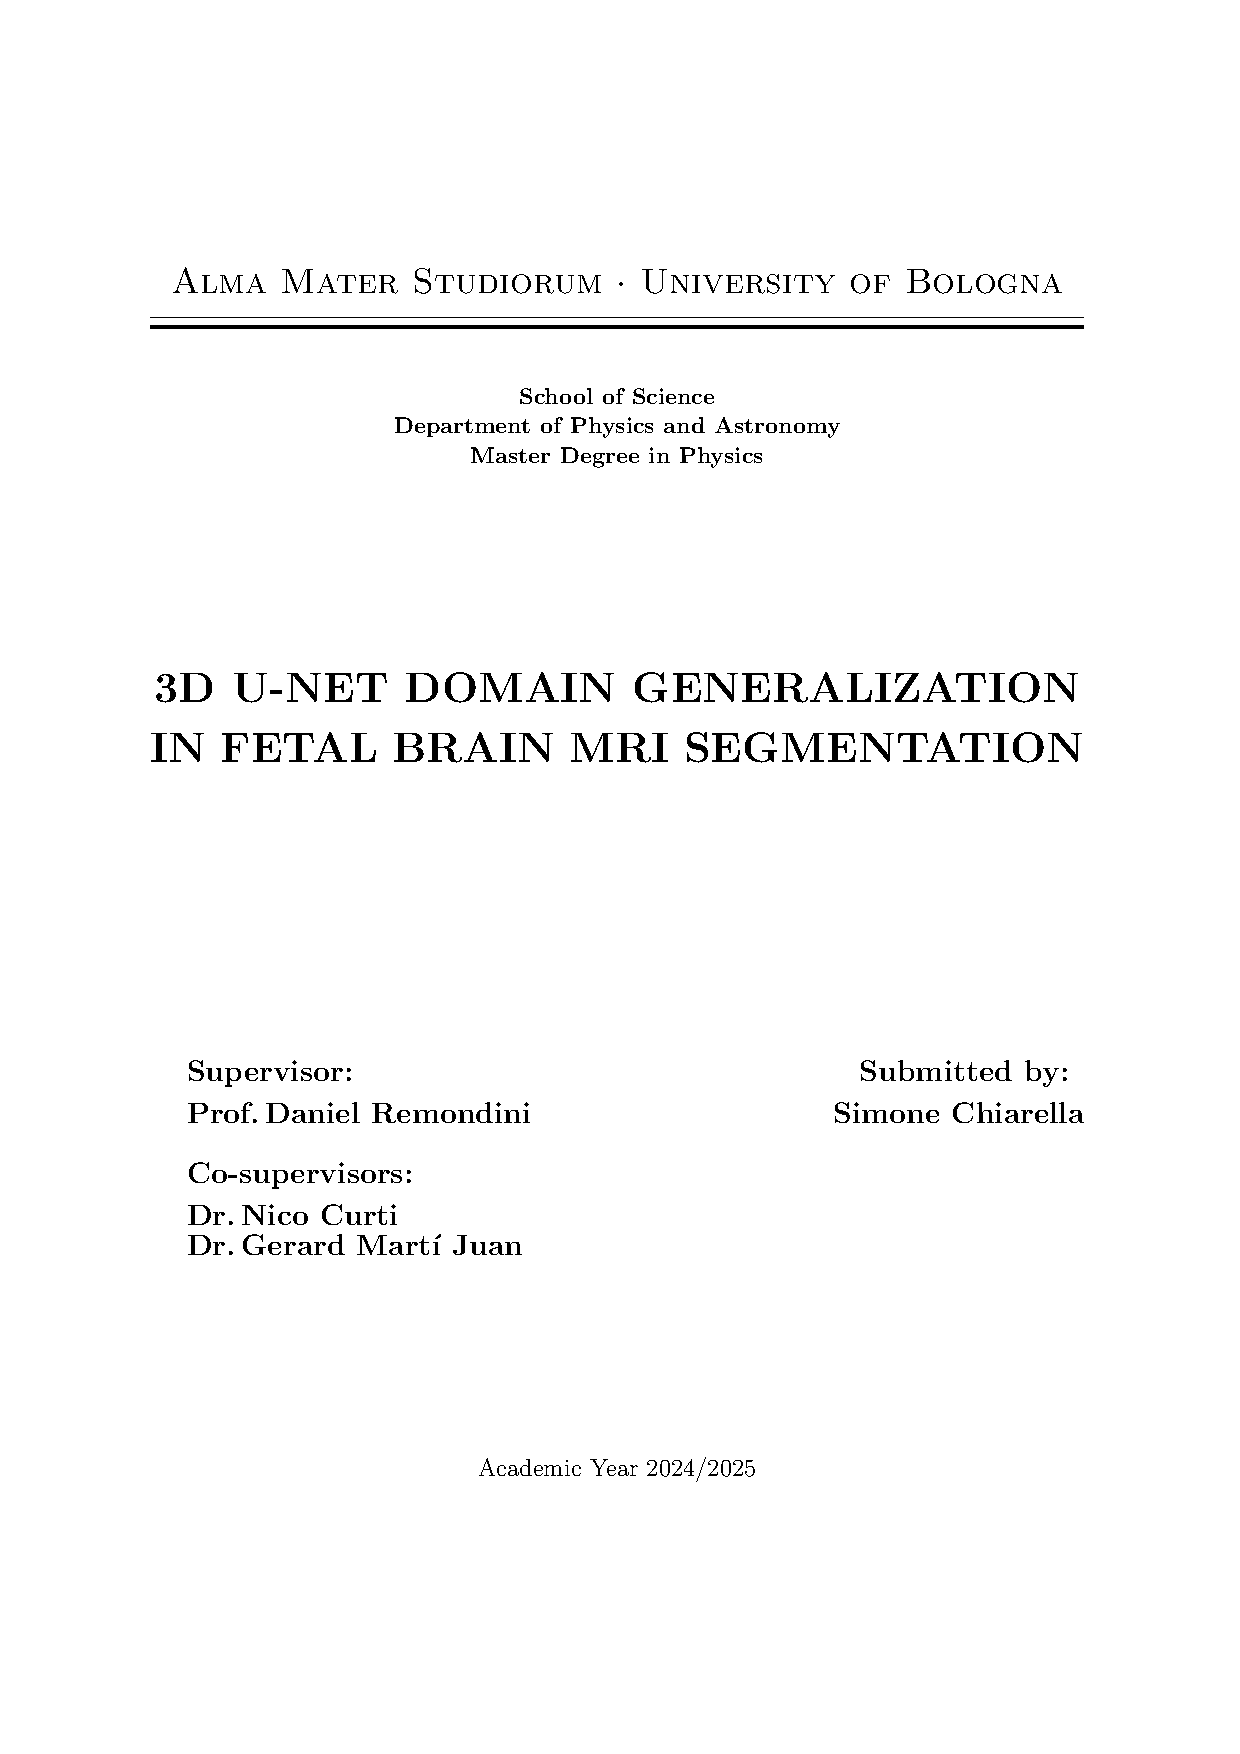
\includepdf[pages=-]{sources/TitlePage.pdf}

\comment{ % This is a hack to move the text block towards the outer border
  \makeatletter
  \if@twoside % commands below work only for twoside option of \documentclass
    \setlength{\textblockoffset}{12mm}
    \addtolength{\hoffset}{\textblockoffset}
    \addtolength{\evensidemargin}{-2.0\textblockoffset}
  \fi
  \makeatother
}

\frontmatter

  \tableofcontents
  \listoffigures
  \listoftables

\mainmatter

  \part[Introduction]{%
    Introduction\\
    %
    \vspace{1cm}
    %
    \begin{minipage}[l]{\textwidth}
    %
    \textnormal{%
      \normalsize
      %
      \begin{singlespace*}
        \onehalfspacing
        %
        Type here the introduction to the part.
      \end{singlespace*}
    }
    \end{minipage}
  }

  %%%%%%%%%%%%%%%%%%%%%%%%%%%%%%%%%%%%%%%%%%%%%%%%%%%%%%%%%%%%%%%%%%%%%%%%
\chapter{Magnetic Resonance Imaging} \label{chap:MagneticResonanceImaging}
%%%%%%%%%%%%%%%%%%%%%%%%%%%%%%%%%%%%%%%%%%%%%%%%%%%%%%%%%%%%%%%%%%%%%%%%
\vspace{1cm}

Magnetic resonance imaging (MRI) is one of the most powerful and versatile techniques in modern medical imaging. Its non-invasive nature and the absence of ionizing radiation have established it as a cornerstone in both clinical diagnostics and biomedical research. MRI exploits the fundamental physical interactions between nuclear spins and magnetic fields, providing not only high-resolution structural images, but also access to functional, metabolic, and microstructural information.

This chapter goes through the fundamental concepts of MRI. First, it introduces the underlying physical principles of nuclear magnetic resonance, including spin dynamics, relaxation processes, and signal generation. Second, it describes how spatial encoding is achieved through magnetic field gradients, which allow the reconstruction of three-dimensional images.

\section{Physical Principles}
Magnetic resonance imaging (MRI) is based on the fundamental physical phenomenon of nuclear magnetic resonance (NMR), first demonstrated experimentally by I.\ Rabi in 1938 and later independently verified by Purcell and Bloch in 1946\,\cite{NMR}. NMR describes the resonant interaction between the intrinsic magnetic moment of atomic nuclei and externally applied magnetic fields. This effect enables the observation of nuclear spin behavior through the emission of electromagnetic radiation, providing the physical foundation for MRI, a technique capable of generating high-resolution, non-invasive images of biological tissues.

If a nucleus possesses an intrinsic angular momentum, or spin \vect{I}, the associated magnetic dipole moment is:
\begin{equation}
    \bm{\upmu} = \gamma \vect{I},
\end{equation}
where $\gamma$ is the gyromagnetic ratio, a constant depending on the nucleus. Only nuclei with a nonzero spin quantum number can exhibit magnetic resonance. Actually, nuclei with a integer spins are not able to produce detectable signals in MRI, because their gyromagnetic ratios are much smaller than those of half-integer spins. Among them, in biological tissues, the hydrogen nucleus ($^1$H) is the most suitable for MRI because of its high abundance in water and lipids and its relatively large $\gamma$, which yields strong detectable signals.

The result of an observation of the $z$-component of the angular momentum \vect{I} of a single nucleus in its ground state is an integer or half-integer number $m$ ranging from $-I$ to $+I$, in steps of \num{1}. Thus, $m$ can assume $2I + 1$ distinct values, which implies $2I + 1$ possible values for the measurement of the $z$-component of the magnetic moment
\begin{equation}
    \mu_z = \gamma \hbar m,
\end{equation}
where $\hbar$ is the reduced Planck constant.

Each value of $m$ corresponds to a specific energy level of the nucleus. When a magnetic field $\vect{B_0}$ is applied, these energy levels split due to the Zeeman effect, resulting in a set of discrete energy states. The energy associated with each state is given by
\begin{equation}
    E_m = -\gamma \hbar m B_0.
\end{equation}
In case of $^1$H, which has $I = \frac{1}{2}$, the two possible values of the magnetic moment correspond to $m = +\frac{1}{2}$ and $m = -\frac{1}{2}$. This results, in turn, in two distinct energy states separated by $\Delta E = \gamma \hbar B_0$. The presence of discrete energy levels generates an observable quantity named magnetization \vect{M}, which is defined as
\begin{equation}
    \vect{M} = N \gamma \hbar (\langle I_x \rangle \vect{i} + \langle I_y \rangle \vect{j} + \langle I_z \rangle \vect{k}),
\end{equation}
where $N$ is the number of nuclei with nonzero spin.

At relatively low temperature $T$ (even room temperature) and high magnetic field \vect{B_0}, the magnetization obeys Curie's law\,\cite{curie_law}:
\begin{equation}
    \vect{M_0} = N\frac{\gamma^2 \hbar^2 I(I+1)}{3\mathrm{k}_\mathrm{B} T} \vect{B_0},
\end{equation}
where $\mathrm{k}_\mathrm{B}$ is the Boltzmann constant. It is important to notice that stronger magnetic fields or lower temperatures increase the detectable magnetization.

The last fundamental principle of NMR is a phenomenon, known as Larmor precession, which originates from the application of an external magnetic field to nuclei with nonzero spin. The magnetic moments $\bm{\upmu}$ of the nuclei will not just align with the direction of the magnetic field, but they will describe a conical motion around \vect{B_0} (Fig.\,\ref{fig:larmor_precession}), at the Larmor frequency:
\begin{equation}
    \nu_\textrm{L} = \frac{\omega_\textrm{L}}{2\uppi} = \frac{\gamma B_0}{2\uppi}.
\end{equation}
To perturb the equilibrium state and generate a measurable signal, a second oscillating magnetic field \vect{B_1}, also called radiofrequency (RF) pulse, is applied perpendicularly to \vect{B_0}. If the oscillation frequency of \vect{B_1} matches $\omega_\mathrm{L}$, resonance occurs and the nuclei absorb energy, undergoing transitions between the energy levels. As a consequence, an increasing nutation angle appears, causing the magnetization \vect{M} to tilt away from the $z$-axis by a flip angle $\alpha$, defined as
\begin{equation}
    \alpha = \gamma B_1 t,
\end{equation}
where $t$ is the duration of the RF pulse. Typical pulses of $90$° or $180$° rotate the magnetization fully into the transverse plane or invert it, respectively.

\section{Spatial Encoding}


  %%%%%%%%%%%%%%%%%%%%%%%%%%%%%%%%%%%%%%%%%%%%%%%%%%%%%%%%%%%%%%%%%%%%%%%%
\chapter{Fetal Brain MRI} \label{chap:FetalBrainMRI}
%%%%%%%%%%%%%%%%%%%%%%%%%%%%%%%%%%%%%%%%%%%%%%%%%%%%%%%%%%%%%%%%%%%%%%%%
\vspace{1cm}

Magnetic resonance imaging is an indispensable tool for the study of the developing human brain, thanks to its non-invasive nature. In the prenatal context, MRI enables the assessment of brain structures that are critical for monitoring neurodevelopment and detecting abnormalities, making fetal brain MRI a cornerstone in both clinical and research settings.

The developing brain presents features that evolve rapidly throughout gestation, requiring imaging protocols tailored to capture fine structural details while minimizing motion-related artifacts. Standardized acquisition protocols, combined with advanced post-processing techniques such as super-resolution reconstruction, are essential to obtaining images of sufficient quality for clinical diagnosis and quantitative analysis. Additionally, adequate parcellation of fetal brain structures is fundamental for studying developmental trajectories and for training automated segmentation models.

Despite these advances, fetal brain MRI remains technically challenging. Factors such as spontaneous fetal motion, maternal respiration, and variability in scanner hardware or acquisition settings introduce significant heterogeneity in the acquired data. This variability has implications not only for clinical interpretation but also for the development of automated tools, which must generalize across diverse imaging conditions.

The present chapter provides an overview of the aforementioned key aspects, presenting the main brain structures of interest during fetal development, alongside typical acquisition and parcellation protocols. Then, the most popular and effective super-resolution reconstruction algorithms are discussed. Finally, it summarizes the current challenges in the field of automated fetal brain segmentation.

\section{Fetal Brain Structures}

\section{Acquisition Protocols}

\section{Parcellation Protocols}

\section{Super-Resolution Reconstruction} \label{sec:SuperResolutionReconstruction}

\section{Challenges} \label{sec:Challenges}
MRI, and in particular fetal brain MRI, presents some characteristics that contribute to significant domain shifts, compromising the performance of deep learning models on unseen data distributions\,\cite{FeTA2024_paper, FeTA2024_review}.

On the biological aspect, the fetal brain is very challenging \textit{per se}, since it undergoes rapid and complex changes throughout gestation:
\begin{description}
    \item[Rapid Morphological Evolution] The brain structure and appearance reorganize dramatically during prenatal development\,\cite{FeTA2024_paper, Ciceri2023}. Defining and consistently identifying different brain structures across varying gestational ages is difficult due to ongoing neuronal migration, gyrification, and sulcation patterns. This means that images acquired at different GAs constitute distinct sub-domains, making a single model challenging to generalize across the entire gestational spectrum\,\cite{Ciceri2024}.
    \item[Low Tissue Contrast] The fetal brain shows different tissue contrast compared to postnatal brains. Specifically, the intensity difference between white matter and gray matter is reduced due to the absence of myelin in the fetal WM. This causes WM to appear brighter than GM on T2w images\,\cite{Ciceri2023}. Tissue contrast changes are also significantly influenced by gestational age\,\cite{FeTA2024_paper}.
    \item[Pathological Heterogeneity] Congenital disorders introduce further significant morphological variations. Training segmentation algorithms exclusively on neurotypical samples can reduce their robustness when encountering altered morphologies typical of pathological cases (e.g., spina bifida, ventriculomegaly, corpus callosum malformations). The rarity and wide variability of fetal pathologies contribute to the challenge of obtaining sufficient data for exhaustive datasets\,\cite{FeTA2024_paper, FeTA2024_review}.
\end{description}

On the technical side, the nature of \textit{in-utero} MRI introduces further limitations\,\cite{Ciceri2023}:
\begin{description}
    \item[Motion Artifacts] Spontaneous fetal movement and maternal breathing during MRI acquisition lead to various artifacts, such as in-plane image blur, slice crosstalk and incongruence in slice location, significantly degrading the quality of individual slices and the reconstructed volume. While ultrafast 2D sequences (e.g., \textsc{ssfse}, \textsc{haste}) are commonly employed to minimize these effects by acquiring each slice rapidly, they cannot entirely eliminate motion-related issues.
    \item[Low Contrast-to-Noise Ratio] The small size of the fetal brain and the need for shorter scanning periods to minimize motion contribute to a low CNR. This, coupled with acquisition limits such as thick slices---to achieve good SNR---, makes it difficult to distinguish fine anatomical details.
    \item[Intensity Inhomogeneities] Radiofrequency field inhomogeneity, non-uniform reception coil sensitivity, eddy currents driven by field gradients, and electromagnetic interactions with the body can cause intensity inhomogeneities. Such variations produce intensity bias fields across the image space, making consistent tissue intensity representation challenging for automated methods.
    \item[Partial Volume Effects] Due to thick slices, a single voxel may contain signals from multiple tissue types. This \enquote{mixing} of signals leads to ambiguous boundaries and can result in mislabeled segmentations, especially at tissue interfaces. For instance, the mixing of the CSF and cortical GM boundary leads to intensities similar to the intensity profile of the WM.
\end{description}

Ultimately, the scarcity of large, standardized, and annotated datasets further jeopardizes the development of robust segmentation algorithms. This is due to\,\cite{FeTA2024_paper,FeTA2021_review, Ciceri2023}:
\begin{description}
    \item[Small and Heterogeneous Cohorts] Fetal MRI studies often require collaboration from specialized clinical centers due to the small and vulnerable patient populations. This leads to small datasets at individual institutions, making it difficult to create uniform in-house single-center datasets.
    \item[Variability in Acquisition Protocols and Hardware] Data from different clinical centers tend to exhibit considerable variability in image acquisition parameters, MRI scanner hardware, and manufacturer specifications. The most important differences use to be in magnetic field strengths (e.g., \qtylist{0.55;1.5;3}{\tesla} and specific sequence parameters (e.g., TR/TE values, flip angles, FOV, slice thickness). The associated acquisition shift cause deep learning models trained on one domain to perform poorly on data from another.
    \item[SR Reconstruction Variability] Fetal MR images are typically acquired as orthogonal stacks of 2D slices to mitigate motion, which then require SR reconstruction algorithms to generate high-resolution 3D volumes. The use of different SRR algorithms (e.g., \textsc{mialsrtk}\,\cite{Tourbier2015, MIALSRTK}, \textsc{irtk}\,\cite{Kuklisova2012, irtk-simple}, \textsc{NiftyMIC}\,\cite{Ebner2020}, \textsc{svrtk}\,\cite{Uus2022}) introduces an additional layer of domain shift.
    \item[Manual Annotation Variability] Creating high-quality, manually labeled data is time-consuming---often taking several hours per case---and requires expert anatomical knowledge. This process is also prone to human error and significant inter-rater variability.
\end{description}

In conclusion, the multifaceted nature of these challenges makes robust and generalizable fetal brain MRI segmentation an exceptionally difficult task. Addressing these domain shifts is paramount for the development of deep learning models aimed to be used in clinical practice for prenatal diagnosis and research.


  %%%%%%%%%%%%%%%%%%%%%%%%%%%%%%%%%%%%%%%%%%%%%%%%%%%%%%%%%%%%%%%%%%%%%%%%
\chapter{Methods for Fetal Brain Segmentation} \label{chap:MethodsForFetalBrainSegmentation}
%%%%%%%%%%%%%%%%%%%%%%%%%%%%%%%%%%%%%%%%%%%%%%%%%%%%%%%%%%%%%%%%%%%%%%%%
\vspace{1cm}

% Type here an introduction to the chapter

\section{Domain Generalization} \label{sec:DomainGeneralization}
In medical image segmentation, a \emph{domain} encapsulates both the feature space and the underlying marginal distribution of imaging data. Domain shifts arise when models trained on one domain are tested on data from another dataset. In medical imaging, the most prevalent sources of domain shift arise from variations in image acquisition processes, encompassing differences in imaging modalities, scanning protocols, and device manufacturers---a more exhaustive description of the potential sources can be found in Section \ref{sec:Challenges}. This is frequently referred to as acquisition shift. Unlike data generalization, where test samples share the same distribution as training data, domain generalization addresses the scenario where test data arise from a distinct, unseen domain\,\cite{Ouyang2023}.

Domain generalization (DG) methods can be categorized into three main groups, which are often complementary and can be combined to achieve higher performance\,\cite{Wang2023}:
\begin{description}
    \item[Data Manipulation] These methods focus on manipulating input data to assist in learning general representations. The primary objective is to increase the diversity and quantity of existing training data.
    \begin{itemize}
        \item \textbf{Data Augmentation-Based DG:} This involves applying various transformations to training data  to simulate different domain characteristics and reduce overfitting. Domain randomization is a common technique where new data is generated by introducing random variations in parameters such as object location, texture, shape, number, illumination, camera view, and noise. An example in medical imaging is SynthSeg\,\cite{Billot2023}, which generates synthetic images with randomized contrasts based on Gaussian mixture models (GMMs), along with geometric deformations and resampling to simulate different image resolutions. FetalSynthSeg\,\cite{Billot2023} further extends this by incorporating intensity clustering and meta-classes for fetal brain MRI. Another approach is adversarial data augmentation, which generates image perturbations that are specifically designed to easily flip the predictions of classifiers, thereby making the model more robust to such changes.
        \item \textbf{Data Generation-Based DG:} It involves creating diverse and rich synthetic data to boost a model's generalization capabilities. Techniques often leverage generative models such as variational auto-encoders (VAEs) and generative adversarial networks (GANs), or strategies like Mixup. These methods can be complex due to their computational demands and the careful design required for the generative models.
    \end{itemize}
    \item[Representation Learning] This category aims to learn feature representations that are robust to domain shifts. The core idea is to decompose the prediction function into a feature extraction (representation learning) function and a classifier function, focusing on making the feature extraction robust.
    \begin{itemize}
        \item \textbf{Domain-Invariant Representation Learning:} This approach seeks to reduce the discrepancies between feature distributions across multiple source domains. The underlying principle is that if feature representations remain invariant to different domains, they are inherently more general and transferable to unseen domains. This can involve methods like kernel-based methods, domain adversarial learning---e.g., domain-adversarial neural networks, DANN---, explicit feature alignment techniques, and invariant risk minimization (IRM).
        \item \textbf{Feature Disentanglement-Based DG:} It aims to separate learned features into domain-shared features---which are common across domains and useful for the task---and domain-specific features---which capture domain-specific variations. In this category, causality-inspired methods aim to ensure that the learned representations capture the \enquote{true cause} of the labels (e.g., object shape) and are therefore unaffected by correlated but irrelevant features like background, color, or style. Causality-inspired methods have been used to achieve single-source domain generalization through data augmentation. The idea is to simulate interventions on irrelevant features, thereby exposing the network to synthetic acquisition-shifted training examples.
    \end{itemize}
    \item[Single-Source Domain Generalization (SSDG)] This is a specific and highly challenging setting within domain generalization where only a single source domain is available for training. This scenario is particularly common in medical imaging applications due to the high cost of data collection, privacy concerns, and scarcity of diverse datasets\,\cite{Ouyang2023}. The key to this problem is to generate novel domains using data generation techniques to increase the diversity and informativeness of training data\,\cite{Wang2023}. The performance degradation that deep learning models face due to domain shift can be attributed to\,\cite{Ouyang2023}:
    \begin{itemize}
        \item \textbf{Shifted Domain-Dependent Features:} Image appearances, including intensities and textures, are inherently domain-dependent. Deep networks are acutely susceptible to shifts in these features. In contrast, human annotators can readily identify anatomical structures across different domains by focusing on domain-invariant shape information, which is intuitively causal to segmentation masks, unlike intensity or texture.
        \item \textbf{Shifted-Correlation Effect:} Due to confounding variables, objects in the background of an image may be spuriously correlated with the objects of interest, rather than causally related. For example, a network might learn that a certain background artifact (which, in the case of fetal MRI, would be the skull and the maternal tissues) is correlated with a specific anatomical structure within a source domain. If this artifact is absent or appears differently in an unseen target domain, the network's reliance on this spurious correlation can lead to failure.
    \end{itemize}
The goal of SSDG is to mitigate these effects by steering the network towards learning domain-invariant features, such as shape information, and immunizing the segmentation model against the shifted-correlation effect by removing confounders during training. This is exactly the idea behind GIN-IPA\,\cite{Ouyang2023}, that is discussed in greater detail in Section \ref{sec:Challenges}.
\end{description}

\section{Atlas-based Methods}

\section{Convolutional Neural Networks}

\section{The FeTA Challenge}
The Fetal Tissue Annotation Challenge (FeTA)\,\cite{FeTA2024} was born in 2020, and joined the International Conference on Medical Image Computing and Computer-Assisted Intervention (\textsc{miccai})\,\cite{MICCAI} in 2021. Up to now, four editions have been organized (in 2020, 2021, 2022, and 2024), with increasing participation and interest from the medical imaging community. The main contributions of the FeTA challenge are the creation of a benchmark dataset for fetal brain MRI segmentation and biometry, and the promotion of the development of algorithms for the automatic segmentation of fetal brain tissues.

The main task in FeTA is the segmentation of brain tissues in fetal MRI, which is a challenging problem due to the low contrast between tissues, the presence of noise, and the variability in the shape and size of the fetal brain. The dataset used in the challenge is composed of 3D super-resolution (SR) reconstructions of 2D fetal brain MRI images. Participants are asked to segment the fetal brain into seven tissues: external cerebrospinal fluid (CSF), cortical gray matter (cGM), white matter (WM), ventricles (including cavum), cerebellum, deep gray matter (dGM), and brainstem (BS). The performance is evaluated using three metrics: the Dice similarity coefficient (DSC), the volume similarity (VS), and the Hausdorff 95 distance (HD95). The use of three metrics helps to reduce the reliance on any one metric, which may be misleading in the evaluation of the algorithms\,\cite{FeTA2024_paper}.

The first edition of the FeTA challenge was organized in 2020, by Payette et al.\,\cite{FeTA2020_review}. The challenge consisted in segmenting fetal brain MRI T2w images. The initial FeTA dataset comprised 40 super-resolution (SR) reconstructions with manual segmentations for training and 10 SR reconstructions without manual segmentation for validation, encompassing both pathological and non-pathological cases. The gestational age (GA) range spanned from 20 to 33 weeks. This dataset established a standard in fetal brain tissue parcellation---according to the seven-tissues protocol previously introduced in\,\cite{Payette2020}---that would be used in all the following FeTA editions. Four research groups participated, submitting a total of ten algorithms. All the algorithms had more or less the same issues in segmenting the CSF---especially for the pathological cases, because of not clear tissue boundaries---and the GM, because of its rapidly changing structure.
The dataset used in the first FeTA edition had important limitations:
\begin{itemize}
    \item Manual segmentations were based on a single segmentation due to time and resource limitations, without consensus delineation.
    \item The data were from one single center, the University Children's Hospital Zurich (Kispi), thus limiting the generalizability of the results.
    \item The images had varying quality grades, with younger GAs and pathological cases often having lower quality.
\end{itemize}

The 2021 edition of the FeTA challenge\,\cite{FeTA2021_review, FeTA2021} was the first to join the \textsc{miccai} conference. The dataset---hereinafter referred to as Kispi dataset---was expanded to 120 scans from the same institution, with GAs ranging from 20 to 35 weeks. The acquisition was carried out at 1.5\,T for a subset of cases, and at 3\,T for another subset of cases. 60 scans were reconstructed with the \textsc{mialsrtk} method\,\cite{Tourbier2015, MIALSRTK}, while the other 60 cases with the \textsc{simple irtk} method\,\cite{Kuklisova2012, irtk-simple}. For each reconstruction method, 40 cases were included in the training dataset available to the challenge participants (for a total of 80 cases), and 20 cases were included in testing dataset not available to the participants (for a total of 40 cases). 21 algorithms were submitted, of which 19 were U-Nets, with no major differences in the architecture. Overall, the most challenging labels to segment were cortical and deep GM---due to limited image resolution and annotation uncertainty---and brainstem---especially in the pathological cases. The results of the image quality and SR reconstruction methods are related to each other, as the majority of the low quality images were done with the \textsc{mialsrtk} method, and the excellent quality brain volumes included were reconstructed with the \textsc{simple irtk} method.

FeTA 2022\,\cite{FeTA2022_review, FeTA2022} introduced a multi-center dataset to address the generalizability of algorithms, which was one of the main limitations of the previous editions. In addition to Kispi, data from Medical University of Vienna was incorporated into both the training and testing datasets. Data from two further centers were included in the testing dataset---University Hospital Lausanne (\textsc{chuv}), and Benioff Children's Hospital (UC San Francisco, \textsc{ucsf})---for a total of four centers (Tab\,\ref{tab:FeTA2022_dataset}).

\begin{table}[htbp]
    \centering
    \begin{tabular}{c|c|c|c|c}
    \toprule
    \textbf{Inst.} & \begin{tabular}{@{}c@{}} \textbf{Scanner} \\ \textbf{(field strength in Tesla)} \end{tabular} & \textbf{SRR method} & \begin{tabular}{@{}c@{}} \textbf{TR/TE} \\ \textbf{(ms)} \end{tabular} & \begin{tabular}{@{}c@{}} \textbf{GA range} \\ \textbf{(weeks)} \end{tabular} \\ \midrule
    \multicolumn{5}{c}{\textbf{Training}} \\
    \midrule
    Kispi & \begin{tabular}{@{}c@{}} GE Signa Discovery \\ MR450/MR750 (1.5/3)* \end{tabular} & \begin{tabular}{@{}c@{}} \textsc{mialsrtk} (40) \\ \textsc{simple irtk} (40) \end{tabular} & \begin{tabular}{@{}c@{}} 2000-3500 \\ 120** \end{tabular} & 20.0-34.8 \\ \hline
    Vienna & \begin{tabular}{@{}c@{}} Philips Ingenia/Intera (1.5) \\ Philips Achieva (3) \end{tabular} & \textsc{NiftyMIC} (40) & \begin{tabular}{@{}c@{}} 6000-22000 \\ 80-140 \end{tabular} & 19.3-34.4 \\
    \midrule
    \multicolumn{5}{c}{\textbf{Testing}} \\
    \midrule
    Kispi & \begin{tabular}{@{}c@{}} GE Signa Discovery \\ MR450/MR750 (1.5/3)* \end{tabular} & \begin{tabular}{@{}c@{}} \textsc{mialsrtk} (20) \\ \textsc{simple irtk} (20) \end{tabular} & \begin{tabular}{@{}c@{}} 2000-3500 \\ 120** \end{tabular} & 21.3-34.6 \\ \hline 
    Vienna & \begin{tabular}{@{}c@{}} Philips Ingenia/Intera (1.5) \\ Philips Achieva (3) \end{tabular} & \textsc{NiftyMIC} (40) & \begin{tabular}{@{}c@{}} 6000-22000 \\ 80-140 \end{tabular} & 18.1-35.0 \\ \hline
    \textsc{chuv} & \begin{tabular}{@{}c@{}} Siemens \textsc{magnetom} \\ Aera (1.5) \end{tabular} & \textsc{mialsrtk} (40) & \begin{tabular}{@{}c@{}} 1200 \\ 90 \end{tabular} & 21.0-35.0 \\ \hline
    \textsc{ucsf} & \begin{tabular}{@{}c@{}} GE Discovery \\ MR750/MR750W (3) \end{tabular} & \textsc{NiftyMIC} (40) & \begin{tabular}{@{}c@{}} 2000-3500 \\ 100** \end{tabular} & 20.0-35.1 \\
    \bottomrule
    \end{tabular}
    \caption{Training and testing dataset properties in FeTA 2022. In parenthesis, next to each SRR method, is reported the correspondent number of images. *The field strengths respectively refers to the scanners. **TE values represent the minimum durations.}
    \label{tab:FeTA2022_dataset}
    \end{table}

17 algorithms were submitted, among which nnU-Net was the most used and effective tool. Overall, the median performance metrics in the OOD setting remained equivalent to the in-domain, but for some labels---ventricles, GM and  WM---an important drop in performance was observed. The most challenging labels to segment remained cortical and deep GM, and BS. Notably, some algorithms performed better in the OOD setting than in the in-domain setting. This can be explained with the better quality of the images from the \textsc{chuv} and \textsc{ucsf} centers, which were included only in the test set. Style and photometric augmentations (contrast, blur, sharpness, etc.) turned out to be effective in improving the generalization of the models. However, \enquote{the optimum choice of augmentation techniques remains unclear}\,\cite{FeTA2022_review}, standing as a critical factor in achieving domain generalization. The paper traces a path for future research, highlighting that it should focus on enhancing the generalizability of the methods and that \enquote{conducting a more comprehensive evaluation of the impact of data augmentation and possible biases due to super-resolution reconstruction methods would be very valuable}\,\cite{FeTA2022_review}.

Finally, in FeTA 2024\,\cite{FeTA2024_review, FeTA2024} 20 new scans were added to the test set, in order to have more results on the OOD performance. These scans were acquired at St.\ Thomas Hospital (King's College London, KCL), with field strength of 0.55\,T (Siemens \textsc{magnetom} Free.Max)\,\cite{FeTA2024_paper}. This decision follows the recent rise in popularity of low-cost low-field MRI systems\,\cite{Aviles2023}, which are particularly suitable for fetal imaging due to their lower SAR and acoustic noise\,\cite{Ponrartana2023}. 16 algorithms were submitted, of which nine were based on nnU-Net\,\cite{nnUNet, Isensee2021}. The top team used an nnU-Net with a denoising autoencoder, generating ensemble predictions from different models. The second top team used a custom U-Net variant, training it on real and synthetic data (SynthSeg\,\cite{Billot2023}), and applying post-processing to discard non-brain tissues from the predictions. All top-three teams applied extensive data augmentation, combinations of standard augmentations, and model ensembling.

Across the leading methods, average DSC plateaued between 0.80 and 0.82, likely due to the quality of both SRR algorithms and manual segmentations\,\cite{FeTA2022_review}. No statistically significant improvement was observed in overall segmentation performance metrics over the last three editions, suggesting that a performance plateau has been reached despite the increasing sophistication of methodologies and dataset diversity. These results indicate that merely architectural modifications are unlikely to produce significant improvements, consistent with observations from other challenges in which U-Net-based methods frequently outperform more complex designs\,\cite{Eisenmann2023, FeTA2024_review}. Notably, the low-field MRI dataset from KCL achieved the highest segmentation performance among all sites. Conversely, the Kispi dataset, in spite of being an in-domain dataset, exhibited the lowest performance. Although domain shifts are widely recognized as a key challenge for deep learning methods in medical imaging\,\cite{Dockes2021}, the sources of these shifts are rarely disentangled. Analysis of domain shifts revealed that image quality was the most influential factor affecting model generalization, leading to Dice score differences of up to 0.10 between low- and high-quality scans. The choice of the SRR pipeline also exerted a substantial impact on segmentation performance, highlighting the need for better modeling of artifacts specific to fetal brain SR pipelines\,\cite{Sanchez2024}. Other factors, such as gestational age, pathology, and acquisition site, contributed marginally to performance variability.

\comment{
\begin{figure}[htbp]
    \centering
    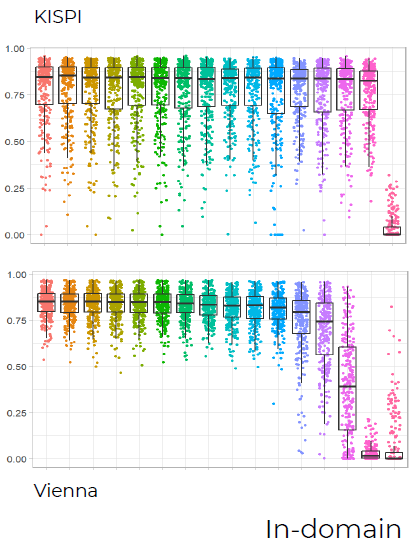
\includegraphics[width=0.4\textwidth]{figures/feta24_in-domain.png}
    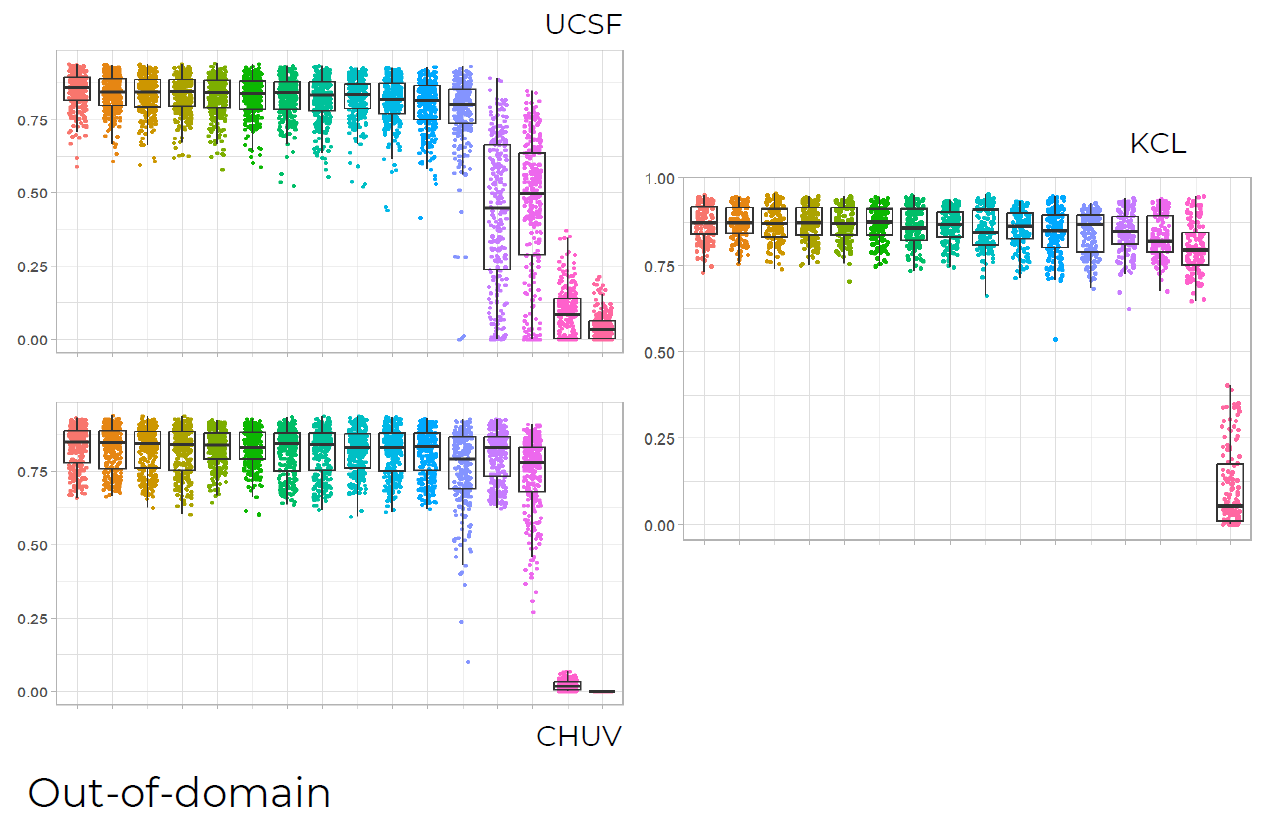
\includegraphics[width=0.8\textwidth]{figures/feta24_out-of-domain.png}
    \caption{Teams' Dice similarity scores in FeTA 2024. From\,\cite{FeTA2024}.}
    \label{fig:FeTA2024_results}
\end{figure}
}

  \part[Materials and Methods]{%
    Materials and Methods\\
    %
    \vspace{1cm}
    %
    \begin{minipage}[l]{\textwidth}
    %
    \textnormal{%
      \normalsize
      %
      \begin{singlespace*}
        \onehalfspacing
        %
        Type here the introduction to the part.
      \end{singlespace*}
    }
    \end{minipage}
  }

  %%%%%%%%%%%%%%%%%%%%%%%%%%%%%%%%%%%%%%%%%%%%%%%%%%%%%%%%%%%%%%%%%%%%%%%%
\chapter{Data} \label{chap:Data}
%%%%%%%%%%%%%%%%%%%%%%%%%%%%%%%%%%%%%%%%%%%%%%%%%%%%%%%%%%%%%%%%%%%%%%%%
\vspace{1cm}

In this study data from two datasets were employed: Kispi and dHCP. While details are provided in the respective sections, an overview is presented in Tab.\,\ref{tab:datasets}.
\begin{table}[hbtp]
    \centering
    \begin{tabular}{c|c|c|c|c|c|c}
        \toprule
        \textbf{Name} & $\textbf{N}_\textbf{n}$\textbf{/}$\textbf{N}_\textbf{p}$ & \makecell{\textbf{GA range} \\ \textbf{(weeks)}} & \makecell{\textbf{Field} \\ \textbf{strength}} & \textbf{Scanner} & \textbf{SRR} & \textbf{Parcel.} \\
        \midrule
        Kispi-mial & 15/25 & 20.0--32.8 & 1.5/3\,T* & \makecell{GE Signa \\ Discovery \\ MR450/750*} & \makecell{\textsc{mialsrtk} \\ \cite{Tourbier2015}} & 7 labels \\ \hline
        Kispi-irtk & 16/24 & 20.01--34.8 & 1.5/3\,T* & \makecell{GE Signa \\ Discovery \\ MR450/750*} & \makecell{\textsc{irtk} \\ \cite{Kuklisova2012}} & 7 labels \\ \hline
        dHCP & 267/0 & 20.9--38.3 & 3\,T & \makecell{Philips \\ Achieva} & \makecell{Cordero- \\ Grande\,\cite{CorderoGrande2018}} & 17 labels \\
        \bottomrule
    \end{tabular}
    \caption{Dataset properties. $\text{N}_\text{n}$ and $\text{N}_\text{p}$ respectively indicates the number of normal and pathological cases. *The field strengths respectively refers to the scanners.}
    \label{tab:datasets}
\end{table}

\section{Kispi}
The Kispi dataset\,\cite{Payette2021, FeTA_MICCAI} originates from the University Children's Hospital of Zurich, Switzerland, in the context of the FeTA challenge. All data were acquired with ethics committee approval from the Canton of Zurich, with research consent provided by the mothers for the use of their data. The dataset is open-access and fully anonymized.

The Kispi cohort comprises fetal brain MRI scans from subjects with both normal and pathological neurodevelopment. The pathological cases include a variety of congenital disorders, such as spina bifida and ventriculomegaly, reflecting a clinically relevant population\,\cite{FeTA2024_paper, Ciceri2024}. The dataset spans a gestational age (GA) range of approximately \numrange{20}{35} weeks. For the FeTA 2024 challenge, the Kispi data was partitioned into a training set of \num{80} volumes and a test set of \num{40} volumes, but only the training set is publicly available. The training partition consists of \num{31} neurotypical and \num{49} pathological cases\,\cite{FeTA2024_review}.

All imaging was performed on \qty{1.5}{\tesla} and \qty{3}{\tesla} GE Signa Discovery (MR450 and MR750) whole-body scanners. The acquisitions were conducted without the use of maternal or fetal sedation. Depending on the specific case, either an 8-channel cardiac coil or a standard body coil was employed\,\cite{FeTA2024_paper}. Acquisition details for the single volumes are not available.

The acquisition protocol consisted of T2-weighted single-shot fast spin-echo (\textsc{ssfse}) sequences acquired in the axial, coronal, and sagittal planes relative to the fetal brain. Key sequence parameters were maintained as follows\,\cite{FeTA2024_paper}:
\begin{itemize}
    \item \textbf{Repetition Time (TR):} \qtyrange[range-units = single, range-phrase = --]{2000}{3500}{\milli\second}.
    \item \textbf{Echo Time (TE):} \qty{120}{\milli\second} (minimum).
    \item \textbf{Flip Angle:} \qty{90}{\degree}.
    \item \textbf{Acquisition Resolution:} An in-plane resolution of \qtyproduct[product-units = power]{0.5 x 0.5}{\milli\meter} with a slice thickness ranging from \qtyrange[range-units = single]{3}{5}{\milli\meter} was employed.
    \item \textbf{Field of View and Matrix Size:} The FOV (\qtyrange[range-units = single, range-phrase = --]{200}{240}{\milli\meter}) and image matrix (\qty{1.5}{\tesla}: \numproduct{256 x 224}; \qty{3}{\tesla}: \numproduct{320 x 224}) were adjusted according to the GA and size of the fetus.
\end{itemize}

Prior to reconstruction, all acquired images for a given subject underwent a manual quality review to compile a stack of suitable scans, with at least one brain scan in each orientation. Each image stack was then reoriented to a standard anatomical plane, and a semi-automated method was used to generate the masks of the single labels in the fetal brain. Segmentations were then inspected and refined. Following these pre-processing steps, the data were processed using one of two distinct SR reconstruction pipelines, resulting in two sub-cohorts within the Kispi dataset. The parcellation distinguishes 7 labels: external cerebrospinal fluid (CSF), cortical gray matter (cGM), white matter (WM), ventricles (including cavum), cerebellum, deep gray matter (dGM), and brainstem (BS)\,\cite{FeTA2024_paper}.

\num{40} image stacks, that is, half of the available Kispi stacks, was processed using the \textsc{mial} Super-Resolution Toolkit (\textsc{mialsrtk}) pipeline\,\cite{Tourbier2015, MIALSRTK}. An example of this group of volumes---from now on referred to as the \enquote{Kispi-mial} sub-cohort---is shown in Fig.\,\ref{fig:kispi-mial_images}. The remaining \num{40} stacks were reconstructed using a pipeline based on the Image Registration Toolkit (\textsc{irtk})\,\cite{Kuklisova2012, irtk-simple}. For this sub-cohort---from now on referred to as the \enquote{Kispi-irtk}---an example is shown in Fig.\,\ref{fig:kispi-irtk_images}.

For both SRR methods the resulting 3D volumes have an isotropic resolution of \qtyproduct[product-units = power]{0.5 x 0.5 x 0.5}{\milli\metre}; scans were standardised to \numproduct{256 x 256 x 256} voxels\,\cite{FeTA2021_review}. The distributions of GA, pathology and image quality of both sub-cohorts are shown in Fig.\,\ref{fig:kispi_plots}. However, the image quality for each volume is not provided in the open-access data, as it is only available as a plot in \cite{FeTA2024_review}. More details about the SR algorithms are given in Section \ref{sec:SuperResolutionReconstruction}.

\begin{figure}[hbt]
    \centering
    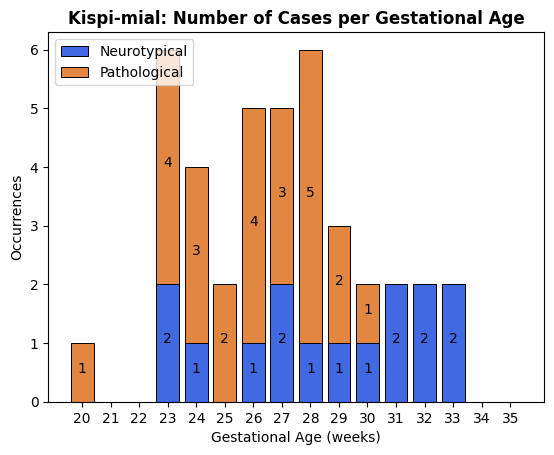
\includegraphics[width=0.45\textwidth]{figures/k-mial_GA.png} \quad
    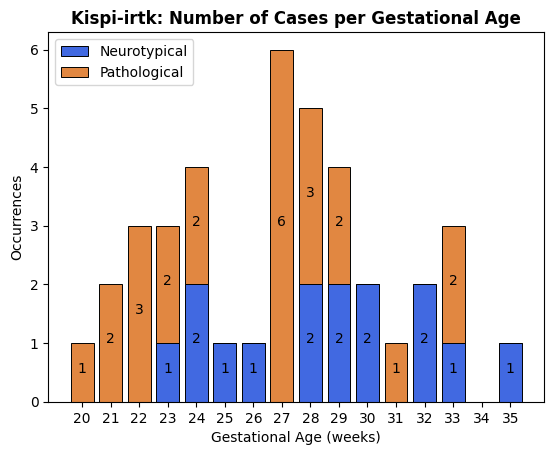
\includegraphics[width=0.45\textwidth]{figures/k-irtk_GA.png}\\
    \vspace{10pt}
    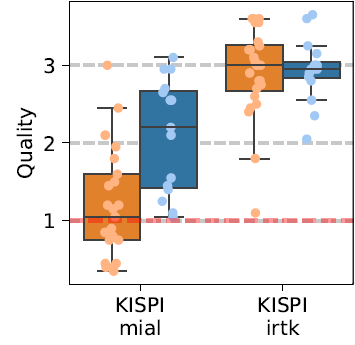
\includegraphics[width=0.32\textwidth]{figures/kispi_quality.png}
    \caption{Top: Kispi cases gestational age distribution, stratified by health condition. Bottom: Quality assessment of Kispi cases, from \cite{FeTA2024_review}.}
    \label{fig:kispi_plots}
\end{figure}

\begin{figure}[hbtp]
    \vspace{-10pt}
    \centering
    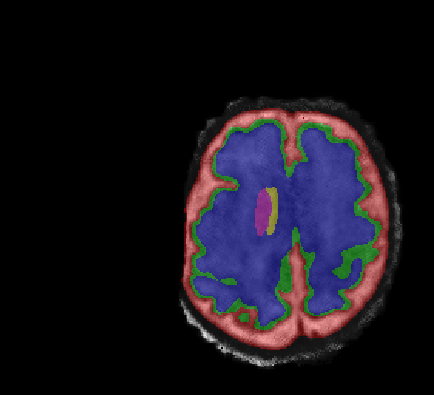
\includegraphics[width=0.33\textwidth]{figures/mial_ax_dseg.png}
    \hspace{5pt}
    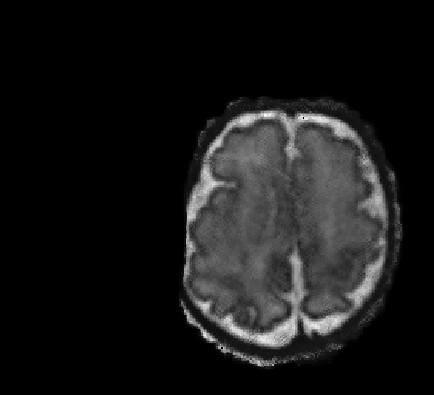
\includegraphics[width=0.33\textwidth]{figures/mial_ax.png} \\
    \vspace{10pt}
    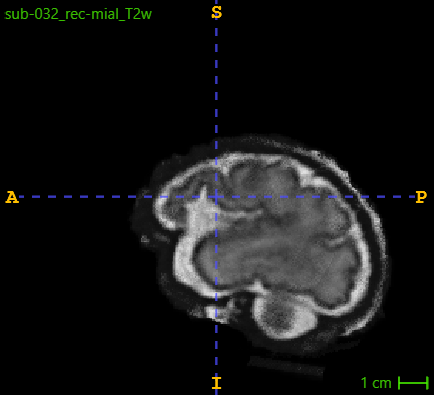
\includegraphics[width=0.33\textwidth]{figures/mial_sag.png}
    \hspace{5pt}
    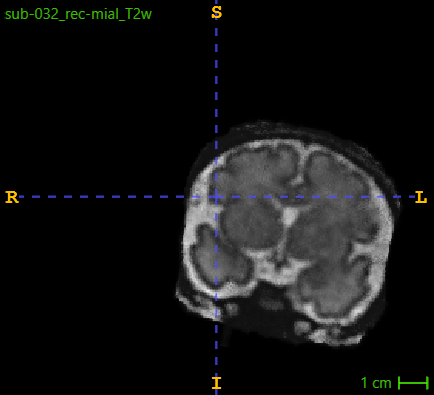
\includegraphics[width=0.33\textwidth]{figures/mial_cor.png}
    \caption{Example of Kispi-mial scan: axial segmentation, axial view, sagittal view, coronal view. Material from: \cite{Payette2021, FeTA_MICCAI}.}
    \label{fig:kispi-mial_images}
\end{figure}
\begin{figure}[hbtp]
    \vspace{-10pt}
    \centering
    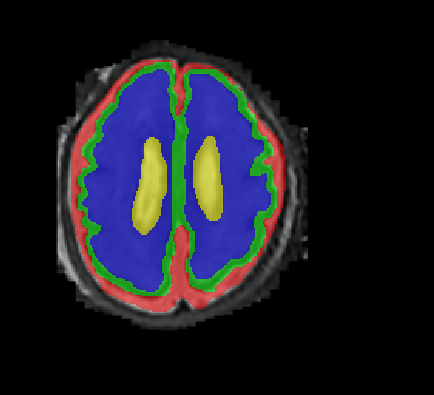
\includegraphics[width=0.33\textwidth]{figures/irtk_ax_dseg.png}
    \hspace{5pt}
    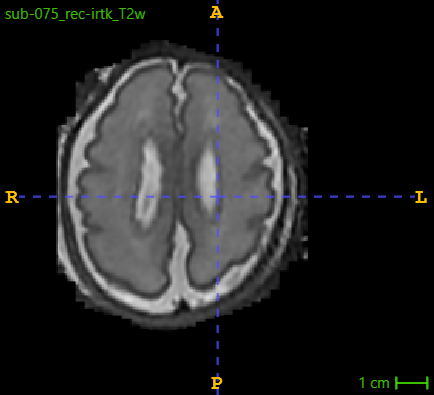
\includegraphics[width=0.33\textwidth]{figures/irtk_ax.png} \\
    \vspace{10pt}
    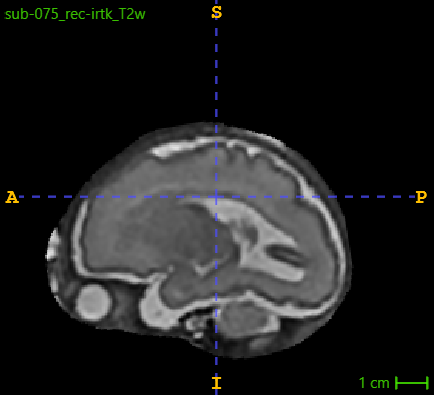
\includegraphics[width=0.33\textwidth]{figures/irtk_sag.png}
    \hspace{5pt}
    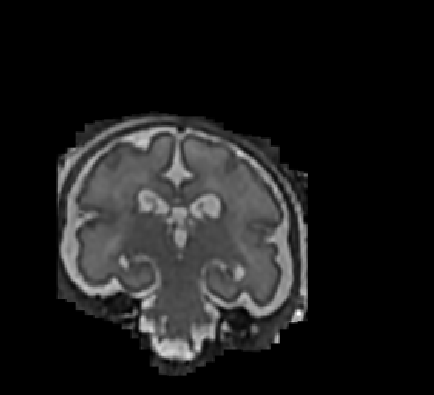
\includegraphics[width=0.33\textwidth]{figures/irtk_cor.png}
    \caption{Example of Kispi-irtk scan: axial segmentation, axial view, sagittal view, coronal view. Material from: \cite{Payette2021, FeTA_MICCAI}.}
    \label{fig:kispi-irtk_images}
    \vspace{-10pt}
\end{figure}

\section{dHCP}
The Developing Human Connectome Project\,\cite{dHCP} (dHCP) provides an open-access spatio-temporal MRI atlas of normal fetal brain development. The dHCP fetal cohort consists of \num{296} scans from \num{272} individuals from St.\ Thomas' Hospital, London, with inclusion based on healthy pregnancies or those without major brain malformations detectable on screening ultrasound. All participants were reported by a neuroradiologist as showing age-appropriate brain anatomy on T2w anatomical scans, with no clinically significant malformations or lesions. The dataset spans a GA range from \numrange{20.86}{38.29} weeks. All imaging was performed on a Philips Achieva \qty{3}{\tesla} using a 32-channel cardiac coil. The distributions of GA and image size are shown in Fig.\,\ref{fig:dhcp_plots}. No sedation was used\,\cite{Karolis2025}.

The dHCP fetal atlas is multi-modal. For each subject, a T2-weighted anatomical scan was acquired during the same session as the functional and diffusion scans. While specific parameters for the structural sequences are not detailed---the most complete description of the fetal structural atlas is reported in an article that actually focuses on funtional MRI\,\cite{Karolis2025}---the final atlas includes T2w and T1w structural channels.

The final structural atlas was constructed from multiple 2D scans combined into high-resolution 3D volumes. Raw 2D slice data were reconstructed into isotropic 3D volumes using slice-to-volume registration (SVR), following the method illustrated in \cite{CorderoGrande2018}. The resulting volumes have a high isotropic resolution of \qtyproduct[product-units = power]{0.5 x 0.5 x 0.5}{\milli\metre}.

The atlas features three parcellations of \numlist{9;17;91} regions of interest. Here, the 17-label parcellation is considered, because it is possible to merge the labels to match exactly the 7-label parcellation used in the Kispi dataset (see Tab.\,\ref{tab:label_merge}). The segmentation is based on the dHCP structural pipeline\,\cite{Makropoulos2018, dHCP_pipeline}---an example is reported in Fig.\,\ref{fig:dhcp_images}. Some ground-truth segmentations are missing, which reduces the number of volumes to \num{267}.

\begin{figure}[hbtp]
    \centering
    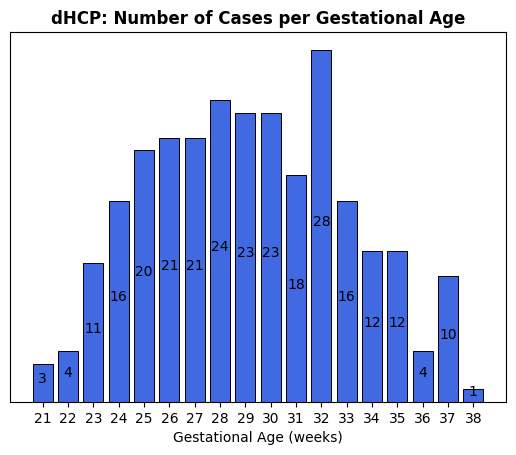
\includegraphics[width=0.5\textwidth]{figures/dHCP_GA.png} \quad
    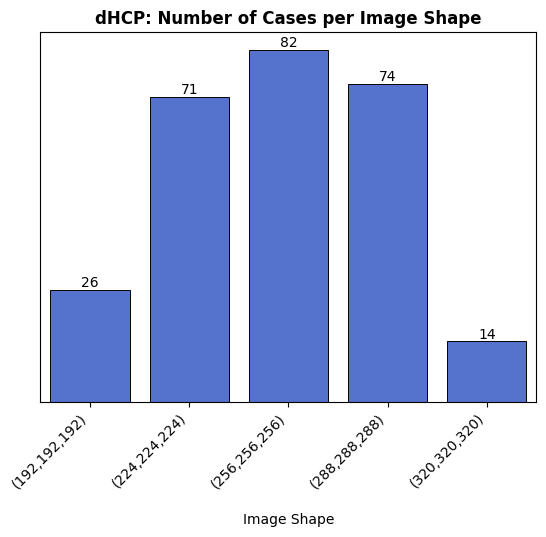
\includegraphics[width=0.44\textwidth]{figures/dHCP_image_shape.png}
    \caption{Distributions of the gestational age and image shape of dHCP cases.}
    \label{fig:dhcp_plots}
\end{figure}
\begin{figure}[hbtp]
    \centering
    \includegraphics[width=0.33\textwidth]{figures/dhcp_ax_dseg.png}
    \hspace{5pt}
    \includegraphics[width=0.33\textwidth]{figures/dhcp_ax.png} \\
    \vspace{10pt}
    \includegraphics[width=0.33\textwidth]{figures/dhcp_sag.png}
    \hspace{5pt}
    \includegraphics[width=0.33\textwidth]{figures/dhcp_cor.png}
    \caption{Example of dHCP scan: axial segmentation, axial view, sagittal view, coronal view. Material from: \cite{dHCP}.}
    \label{fig:dhcp_images}
\end{figure}

\begin{table}[hbtp]
    \centering
    \begin{tabular}{c|c}
        \toprule
        \textbf{Kispi labels} & \textbf{dHCP labels} \\
        \midrule
        1. CSF & 1. Cerebrospinal fluid \\ \hline
        2. cGM & 2. Cortical gray matter \\ \hline
        \multirow{2}{*}{3. WM} & 3. White matter \\
         & 17. Corpus callosum \\ \hline
        \multirow{5}{*}{4. Ventricles} & 4. Left ventricle \\
         & 5. Right ventricle \\
         & 6. Cavum septum \\
         & 15. Third ventricle \\
         & 16. Fourth ventricle \\ \hline
        \multirow{3}{*}{5. Cerebellum} & 8. Left cerebellum \\
         & 9. Right cerebellum \\
         & 10. Vermis \\ \hline
        \multirow{4}{*}{6. dGM} & 11. Left nucleus caudatus and putamen \\
         & 12. Right nucleus caudatus and putamen \\
         & 13. Left thalamus \\
         & 14. Right thalamus \\ \hline
        7. BS & 7. Brainstem \\
        \bottomrule
    \end{tabular}
    \caption{Conversion table between Kispi and dHCP labels.}
    \label{tab:label_merge}
\end{table}

\section{Data Specifications}

  
  %%%%%%%%%%%%%%%%%%%%%%%%%%%%%%%%%%%%%%%%%%%%%%%%%%%%%%%%%%%%%%%%%%%%%%%%
\chapter{Methods} \label{chap:Methods}
%%%%%%%%%%%%%%%%%%%%%%%%%%%%%%%%%%%%%%%%%%%%%%%%%%%%%%%%%%%%%%%%%%%%%%%%
\vspace{1cm}

This chapter describes the methods employed in the present work for fetal brain MRI segmentation and evaluation. The focus is on the domain generalization of deep learning models.

It starts with an overview of nnU-Net, a self-configuring U-Net-based framework that has become a widely adopted baseline in medical image segmentation. Building on this baseline, the method \textsc{gin-ipa} is introduced as an augmentation strategy to enhance domain generalization. Finally, to objectively assess model performance a set of evaluation metrics is presented, based on segmentation accuracy. These include overlap-based measures such as the Dice coefficient, as well as surface-distance-based metrics that capture geometric fidelity.

\section{nnU-Net} \label{sec:nnUNet}
nnU-Net\,\cite{Isensee2021, nnUNet} is an automated pipeline for the tissue segmentation in a task-agnostic configuration, that is, nnU-Net is designed to be applicable to a wide variety of target structures and image properties. Its self-configuring nature allows it to be applied to arbitrary new datasets without manual intervention. nnU-Net does not introduce new elements in the network architecture, but by systematizing the complex process of manual tuning it manages to achieve an automated and efficient setting of parameters in U-Net architecture. This generalized choice of pipeline parameters is carried out based on a \enquote{dataset fingerprint}, that is \enquote{a standardized dataset representation comprising key properties}\,\cite{Isensee2021} of the images. The parameter setting strategy is based on distinguishing between three classes of parameters that can be optimized:
\begin{description}
    \item[Fixed parameters] A robust and consistent choice of hyperparameters and design implementation that is suitable for any task and dataset---they can still be manually changed though. Examples are learning rate, loss function, optimizer, training and testing procedure.
    \item[Rule-based parameters] They are set based on the information taken from the dataset fingerprint, which is acquired during the preprocessing step. This information is fed into rules to automatically make several choices, such as patch and batch size, network topology, intensity normalization, and resampling strategy.
    \item[Empirical parameters] Limited to the choice of the U-Net configuration (2D, 3D-fullres, 3D-cascade) and post-processing.
\end{description}
The rules established generate the same set of parameters and architecture when the image size and the pixel spacing are the same or similar. Default preprocessing consists in cropping the image around non-zero voxels and performing \textit{z}-normalization.

Data augmentation in nnU-Net consists of a set of standard transformations: flip, rotation, scaling, Gaussian noise and blur, resolution reduction, brightness and contrast adjustments, and gamma transformation\,\cite{nnUNet}. Each transformation is applied randomly with a predetermined, empirically chosen probability\,\cite{Isensee2021}.

nnU-Net is currently one of the most popular tools for MRI fetal brain tissue segmentation, representing the state of the art in this field. Nevertheless, like other methods it suffers drops in performance, especially when it comes to inference on out-of-domain (OOD) images and on specific labels, like ventricles, gray matter and white matter.

\section{GIN-IPA} \label{sec:gin-ipa}
To improve robustness of segmentation models against acquisition-induced domain shifts, the causality-inspired augmentation pipeline \textsc{gin-ipa}\,\cite{Ouyang2023} was adopted. The method, that is aimed at single-source domain generalization (see Section \ref{sec:DomainGeneralization}), treats the image formation process as generated by two independent factors, acquisition $A$ and content $C$, and seeks to enforce that the segmentation predictor be invariant to interventions on $A$. Concretely, following the causal formulation, the desired invariance can be expressed as
\begin{equation}\label{eq:domain-inv}
    p\bigl(Y\mid S,\,\mathrm{do}(A= a_i)\bigr) 
    = p\bigl(Y\mid S,\,\mathrm{do}(A= a_j)\bigr), \quad \forall a_i,a_j,
\end{equation}
where $S$ denotes an ideal, domain-invariant representation determined by content $C$---i.e., shape information---and $Y$ is the segmentation mask. $p\bigl(Y\mid S,\,\mathrm{do}(A= a_i)\bigr)$ denotes the distribution that comes from letting images to be generated from a specific acquisition process $A = a_i$---being the same for another acquisition process $A = a_j$.

Because performing real interventions on $A$ is infeasible, \textsc{gin-ipa} approximates such interventions by sampling photometric transformations $T(\cdot)$ that emulate different acquisition processes, and by enforcing consistency of network predictions across these simulated interventions.

The global intensity non-linear augmentation (GIN) module synthesizes a family of non-linear intensity and texture transforms that preserve anatomical geometry while producing diverse appearances (Fig.\,\ref{fig:gin_schema}). Each transform is instantiated as a shallow fully-convolutional network whose weights are sampled from isotropic Gaussian priors and whose inter-layer nonlinearity is a Leaky ReLU. The overall operator is expressed as
\begin{equation}\label{eq:gin}
    g_{\theta}(x) = \frac{\alpha\,g^{\mathrm{Net}}_{\theta}(x) + (1-\alpha)\,x}{\lVert \alpha\,g^{\mathrm{Net}}_{\theta}(x) + (1-\alpha)\,x \rVert_\mathrm{F}}\;\lVert x \rVert_\mathrm{F},
\end{equation}
where $g^{\mathrm{Net}}_{\theta}(\cdot)$ denotes the pure network output for random weights $\theta$, $\alpha\sim\mathcal{U}(0,1)$ is an interpolation coefficient and $\lVert\cdot\rVert_\mathrm{F}$ is the Frobenius norm. The normalization constrains the global energy of the augmented image, preventing global brightness or contrast changes from dominating the image. In other words, it ensures that anatomical shapes remain discernible while still allowing local texture and intensity variations to be introduced.

Key design choices include small receptive fields in the random convolutions (to avoid oversmoothing), linear interpolation with the original image (to retain semantics), and shallow depth (for computational efficiency and to avoid irrealistic results).

\begin{figure}[htbp]
    \centering
    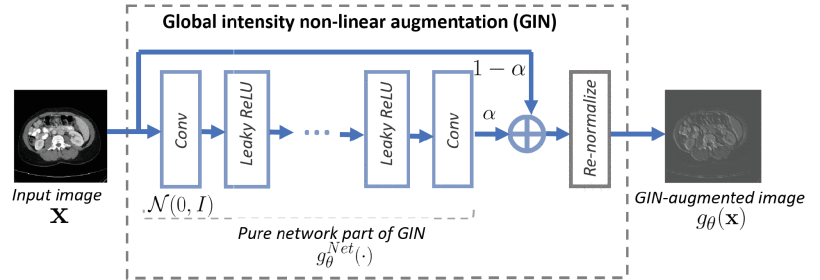
\includegraphics[width=0.9\textwidth]{figures/gin_schema.png}
    \caption{Architecture of the GIN module. © 2022 IEEE, from \cite{Ouyang2023}.}
    \label{fig:gin_schema}
\end{figure}

Then, the interventional pseudo-correlation augmentation (IPA) addresses the shifted-correlation effect, whereby background unlabeled structures $X_\mathrm{b}$ become spuriously correlated with objects of interest $X_\mathrm{f}$ due to the acquisition process. IPA approximates the causal intervention $\mathrm{do}(X_\mathrm{f}=x_\mathrm{f})$---i.e., it removes the effects of the acquisition factor $A$ on $X_\mathrm{f}$---by resampling background appearances independently of the foreground through spatially-varying assignments of appearance transforms.

Let $g_{\theta_1}$ and $g_{\theta_2}$ be two independent GIN transforms sampled for the same input image, with number of channels $C$, height $H$ and width $W$. IPA creates a low-frequency pseudo-correlation map $b\in[0,1]$ with shape $(C \times H \times W)$ and blends the two GIN outputs as
\begin{equation}\label{eq:ipa}
    T_1\bigl(x;\theta_1,\theta_2,b\bigr) = g_{\theta_1}(x) \odot b + g_{\theta_2}(x) \odot (1-b),
\end{equation}
where $\odot$ denotes the Hadamard product, that is, element-wise multiplication. A complementary view $T_2(\cdot)$ is obtained by swapping $b$ and $1-b$. Pseudo-correlation maps are generated by interpolating a lattice of randomly-valued control points with cubic B-splines; in practice the control-point spacing is set to a fraction of the image dimension $\bigl(\textrm{e.g., }\frac{1}{4}\bigr)$ to maintain low spatial frequency and avoid shape distortion (Fig.\,\ref{fig:ipa_schema}).

By applying IPA to the entire image---both background and foreground---the pipeline avoids label-induced shortcuts and approximates sampling from independent background appearance distributions. This operation can be interpreted as assigning different photometric transformations to different spatial regions so that background and foreground appearances are de-correlated across training iterations.

\begin{figure}[htbp]
    \centering
    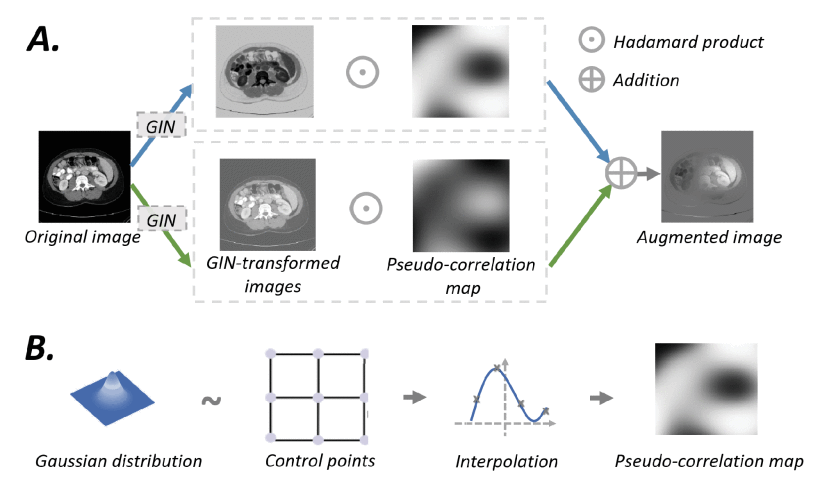
\includegraphics[width=0.9\textwidth]{figures/ipa_schema.png}
    \caption{Architecture of the IPA augmentation scheme (A), and construction principles of pseudo-correlation maps (B). © 2022 IEEE, from \cite{Ouyang2023}.}
    \label{fig:ipa_schema}
\end{figure}

In \cite{Ouyang2023} the training loop samples two GIN transforms and one pseudo-correlation map per image per iteration, generates the two IPA-augmented views $T_1(x)$ and $T_2(x)$, and computes the training loss. Alternative designs to B-spline in pseudo-correlation maps---e.g., random superpixels---were explored but found to be less effective. Both GIN and IPA steps are ruled by hyperparameters that must be set empirically. Among them, the most relevant (followed by the value that was used in \cite{Ouyang2023}, as a reference) are:
\begin{itemize}
    \item GIN
    \begin{itemize}
        \item Number of layers of the shallow network: \num{4}.
        \item Number of intermediate channels of the shallow network: \num{2}.
        \item Interpolation coefficient $\alpha$: sampled from a uniform distribution.
    \end{itemize}
    \item IPA
    \begin{itemize}
        \item Control point spacing in kernel matrix: $\frac{1}{4}\textrm{ of the image length}$; it must be small enough in order to construct low-frequency pseudo-correlation maps.
        \item Interpolation order in kernel matrix: \num{2}, it serves as smoothing factor between the control points in the pseudo-correlation map.
        \item Control point values: sampled from a Gaussian distribution.
        \item Downscale of the image: \num{2}, reduce the computational load.
    \end{itemize}
\end{itemize}
Default values were set by the authors of the paper by the combination of hyperparameter tuning, heuristic choices and hardware limitations.

Actually, practical optimizations include controlling the depth and width of the GIN networks. In \cite{Ouyang2023}, Ouyang and colleagues conducted hyperparameter tuning on the number of layers and channels in the GIN architecture, and on the sampling distribution of the interpolation coefficient $\alpha$. An ablation study on the contribution of the IPA step to the global performance was also conducted, showing improvements in all tested scenarios with respect to GIN-only training.

The proposed approach consistently yields superior performance gains compared with other methods---MixStyle\,\cite{Zhou2021}, AdvBias\,\cite{Chen2020}, RandConv\,\cite{Xu2021} and others---when tested on unseen domains across three cross-domain segmentation scenarios:
\begin{itemize}
    \item Cross-modality abdominal image segmentation (CT-MRI).
    \item Cross-sequence cardiac MRI segmentation (bSSFP-LGE).
    \item Cross-site prostate MRI segmentation.
\end{itemize}

Finally, Ouyang and colleagues also participated in the FeTA 2022 challenge\,\cite{FeTA2022_review}. Their approach was based on training different nnU-Net models with varying data augmentation methods. \textsc{gin-ipa} was employed in the augmentation pipeline for one of these models\,\cite{FeTA2022_top}. The models were subsequently ensembled, and the resulting segmentation method achieved the highest performance in the challenge, ranking first. GIN augmentation and \textsc{gin-ipa} were also used in three models in the FeTA 2024 challenge\,\cite{FeTA2024_review}.

\section{Evaluation Metrics}
To assess the performance of the segmentation models, three evaluation metrics were employed: the Dice similarity coefficient (DSC), the volume similarity (VS), and the 95\th percentile Hausdorff Distance (HD95). These metrics were chosen for consistency with the evaluation protocol adopted in the FeTA challenge\,\cite{FeTA2021_review}.

The Dice similarity coefficient\,\cite{Dice1945,FeTA2021_review} measures the amount of overlap between the manual, ground-truth segmentation $S_\text{g}$ label and the predicted segmentation $S_\text{p}$ generated by the algorithm. It is defined as
\begin{equation}
    \text{DSC}(S_p, S_g) = \frac{2 |S_p \cap S_g|}{|S_p| + |S_g|},
\end{equation}
where $|\cdot|$ denotes the cardinality of a set. The DSC ranges from \num{0} (no overlap) to \num{1} (perfect overlap) and is widely used in medical image segmentation tasks.

The volume similarity measures the relative agreement between the predicted volume $V_\text{p}$ and ground-truth volume $V_\text{g}$. It is defined as
\begin{equation}
    \text{VS}(S_p, S_g) = \frac{2(V_\text{p} - V_\text{g})}{V_\text{p} + V_\text{g}},
\end{equation}
with values closer to \num{0}---both positive and negative---indicating better agreement. Positive values indicate overestimation of the volume of the predicted label, while negative values indicate underestimation. Unlike DSC, VS is sensitive to volumetric discrepancies, regardless of spatial alignment.

The Hausdorff distance\,\cite{Hausdorff1991, FeTA2021_review} evaluates the geometric similarity between two surfaces by measuring the distance between their boundaries. It helps evaluating the contours of segmentations as well as the spatial positions of the voxels. To reduce sensitivity to outliers, the 95\th percentile of all pairwise boundary distances is typically reported:
\begin{equation}
    \text{HD}_{95}(S_p, S_g) = \max \left\{ h_{95}(S_p, S_g), \, h_{95}(S_g, S_p) \right\},
\end{equation}
where $h_{95}(S_\text{p}, S_\text{g})$ is the 95\th percentile of the distances from each boundary point in $S_\text{p}$ to the closest point in $S_\text{g}$.

Together, these three metrics capture complementary aspects of segmentation quality: spatial overlap, volumetric agreement, and boundary accuracy. The metrics were computed using the scikit-image library\,\cite{Walt2014, scikit-image}.

Beyond evaluating segmentation quality with DSC, VS, and HD95, it is essential to assess whether the observed differences between models are statistically significant and to quantify their magnitude. To this end, two complementary statistical tools were employed: the Wilcoxon signed-rank test and Cohen's \textit{d}.

The Wilcoxon signed-rank test\,\cite{Wilcoxon1945} is a non-parametric alternative to the paired \textit{t}-test, used to compare two related samples without assuming normality of their differences. In our case, the test was applied to the paired metric values obtained for the same anatomical structures across the two segmentation methods. The null hypothesis states that the two models have equal performance, while the one-sided alternative tests whether the proposed method achieves superior results. The \textit{p}-value was computed with the function \verb|scipy.stats.wilcoxon|\,\cite{SciPy}.

While statistical significance establishes whether a difference is unlikely to have occurred by chance, it does not provide information on the magnitude of the effect. For this reason, Cohen's \textit{d} effect size\,\cite{Cohen2013} was used, adapted for paired samples. In this formulation, the standardized mean difference is computed on the pairwise differences of the metrics between the metric values of the proposed method and those of the baseline\,\cite{effect_size}:
\begin{equation}
    d = \frac{\mu_1-\mu_2}{\sigma},
\end{equation}
where $\mu_1$ and $\mu_2$ are the means of the proposed method and baseline, respectively, and $\sigma$ is the pooled standard deviation, that for paired samples ($N_1 = N_2$) is:
\begin{equation}
    \sigma = \sqrt{\frac{\sigma_1^2+\sigma_2^2}{2}}.
\end{equation}
Positive values indicate a benefit of the proposed method over the baseline. Cohen's \textit{d} values around \numlist{0.2; 0.5; 0.8} are conventionally interpreted as small, medium, and large effects, respectively.

Together, the Wilcoxon signed-rank test and Cohen's \textit{d} enable a comprehensive comparison: the former addresses the statistical reliability of the observed differences, while the latter quantifies their practical relevance. This dual approach ensures that improvements are not only statistically significant, but also meaningful in terms of segmentation performance.


  %\include{sources/Experimental Strategy}

  \part[Results and Discussion]{%
    Results and Discussion\\
    %
    \vspace{1cm}
    %
    \begin{minipage}[l]{\textwidth}
    %
    \textnormal{%
      \normalsize
      %
      \begin{singlespace*}
        \onehalfspacing
        %
        Type here the introduction to the part.
      \end{singlespace*}
    }
    \end{minipage}
  }

  %\include{sources/...}

  %%%%%%%%%%%%%%%%%%%%%%%%%%%%%%%%%%%%%%%%%%%%%%%%%%%%%%%%%%%%%%%%%%%%%%%%%
\chapter{Discussion} \label{chap:Discussion}
%%%%%%%%%%%%%%%%%%%%%%%%%%%%%%%%%%%%%%%%%%%%%%%%%%%%%%%%%%%%%%%%%%%%%%%%
\vspace{1cm}

This chapter discusses the empirical evidence reported in Chapter \ref{chap:Results}, drawing a unified interpretation across general performance trends across datasets, pairwise model comparisons, and pathology-stratified analyses. The emphasis is on the behavior of the augmentation strategies in realistic in-domain and out-of-domain settings, and on the conditions under which gains are observed.

\section{Primacy of Data over Augmentation}
The first, and most consistent, observation is the primacy of the training dataset over the augmentation recipe. Models trained on dHCP achieve the most stable performance both ID and OOD, and do so \emph{independently} of whether augmentation is the nnU-Net default, GIN-IPA, or their combination. In Section \ref{sec:GeneralPerformance}, this is visible in the DSC histograms (Figs.\,\ref{fig:default_DC}--\ref{fig:both_DC}): while Kispi-trained models experience a marked OOD drop---particularly towards dHCP, with ventricles, dGM and WM most affected---the dHCP-trained models exhibit limited degradation across inference domains. Moreover, no DSC gain emerges from switching augmentation when training on dHCP. Together, these findings imply that \emph{dataset quality and scale} dominate generalization in this setting.

A further confirmation of the importance of the data quality emerges for Kispi-mial: the change of domain does not impact the network trained on Kispi-mial in the same manner as the other two sources. This is partially attributable to the lower image quality in Kispi-mial \cite{FeTA2021_review}. It is therefore expected that any model evaluated OOD on Kispi-mial will underperform relative to other datasets.

\section{Efficacy of GIN-IPA}
\paragraph{Baseline vs.\ GIN-IPA.}
When training on Kispi-irtk and inferring on dHCP, GIN-IPA yields a \emph{substantial improvement} over the baseline across metrics and labels. At the global level, the average DSC increases $(\qty{+58}{\percent})$, with concordant improvements in VS $(\qty{-36}{\percent})$ and HD95 $(\qty{-22}{\percent})$. The corresponding paired analysis confirms the statistical significance and a large effect size for DSC in this cross-domain transfer (DSC: \numrange[range-open-phrase=from\ ]{0.34}{0.54}, $p \ll 0.01$, $|d|=1.1$; VS: \numrange[range-open-phrase=from\ ]{1.12}{0.71}, $p\ll 0.01$, $|d|=0.8$; HD95: \numrange[range-open-phrase=from\ ]{49}{38}, $p\ll 0.01$, $|d|=0.6$). The increase is particularly pronounced for dGM (DSC: \numrange[range-open-phrase=from\ ]{0.18}{0.59}), ventricles (DSC: \numrange[range-open-phrase=from\ ]{0.11}{0.42}), and BS (DSC: \numrange[range-open-phrase=from\ ]{0.43}{0.70}). The full set of paired comparisons for all metrics and labels (including VS and HD95) is reported in Appendix \hyperref[app:SupplementaryTables]{B}.

Conversely, training on dHCP shows no material benefit from GIN-IPA over the baseline across any inference domain or label. For Kispi-mial, effects are small and structure-dependent, with modest improvements predominantly in cases where the baseline struggles on poorly segmented volumes.

\paragraph{GIN-IPA vs.\ Combined Augmentation.}
Stacking the two augmentation methods does not systematically improve performance over GIN-IPA alone. When trained on Kispi-irtk and inferred on dHCP, the combined strategy is consistently inferior to pure GIN-IPA for several structures (CSF, cerebellum, dGM) across all metrics. Training on dHCP again yields no differences between the two.

\section{Robustness by Pathology}
The stratified analysis (Section \ref{sec:PerformanceByPathology}) indicates that models trained on dHCP generalize equally well to healthy subjects in Kispi-mial and Kispi-irtk, despite the domain shift (different image quality and reconstruction techniques). Performance decreases for pathological cases, reflecting segmentation challenges in the presence of anatomical abnormalities. In this more difficult regime, GIN-IPA achieves very small improvements over the baseline, while remaining broadly equivalent to the combined strategy. These results also suggest that the lower-quality images are concentrated among pathological scans, explaining the larger performance gap in that subgroup.

\section{General Outcomes}
The evidence above supports three general conclusions:
\begin{itemize}
    \item \textbf{Data quality and scale prevail:} When training data are abundant and homogeneous (like in dHCP), model choice of augmentation among those tested barely alters performance. The converse is also true: with smaller, noisier sources (such as Kispi), OOD degradation is pronounced.
    \item \textbf{GIN-IPA is conditionally beneficial:} Its gains are largest in the domain generalization scenario from Kispi-irtk to dHCP, where it closes a considerable part of the OOD gap. Effects shrink or vanish when the source dataset already captures the target variability.
    \item \textbf{Stacking augmentations is not additive:} The combined strategy often overlaps with, and can even dilute, the benefits of GIN-IPA; it never consistently outperforms GIN-IPA in the examined cross-domain settings.
\end{itemize}

These patterns are coherent with the intended role of GIN-IPA: by synthesizing intensity and spatial variations, it exposes the network to harder, more diverse views of a limited source, which is most valuable when the source lacks the target domain variability. Once data already cover the relevant distributional modes (as with dHCP), marginal augmentation gains become negligible.

\section{Limitations and Future Work}
Three principal aspects delimit the scope of the present findings. First, the small size of the Kispi cohorts constrained further stratification (e.g., finer gestational age, training by pathology) and limits the precision of subgroup estimates. Generally speaking, the limited availability of public datasets, together with their high intra-variability, jeopardizes the possibility to totally isolate single domains. Second, label-set harmonization between Kispi and dHCP required a mapping (Tab.\,\ref{tab:label_merge}), which, although carefully defined, introduces an additional layer of variability in label-wise comparisons. Third, because of hardware limitations, the IPA step was performed in its 2D variant, which may be less effective than the full 3D version.

Practically, the results argue for prioritizing \emph{data curation}---larger, multi-center, high-quality fetal MRI with standardized SRR pipelines---since source quality and scale are the dominant predictors of cross-domain success in this task. Within constrained-data regimes, GIN-IPA is a \emph{useful augmentation choice}, particularly for single-source DG from moderately sized, relatively clean sources (e.g., Kispi-irtk). Nonetheless, stacking it with standard nnU-Net augmentation is unnecessary and sometimes counterproductive. For challenging pathological cases, improved acquisition and reconstruction remain central to performance gains.

Besides data, it could be interesting to disentangle the two components of GIN-IPA---possibly employing the 3D IPA variant and broader datasets that allow a more rigorous cross-domain validation---to assess their individual contributions, and to explore other augmentation strategies (e.g., adversarial, style-transfer) in this setting.


  \part*{Conclusions}
  \addcontentsline{toc}{part}{Conclusions}

  %\newpairofpagestyles[scrheadings]{conclusions}{\ohead{Conclusions}}
%\thispagestyle{conclusions}
\addcontentsline{toc}{part}{Conclusions}

%%%%%%%%%%%%%%%%%%%%%%%%%%%%%%%%%%%%%%%%%%%%%%%%%%%%%%%%%%%%%%%%%%%%%%%%
\chapter*{Conclusions}
%%%%%%%%%%%%%%%%%%%%%%%%%%%%%%%%%%%%%%%%%%%%%%%%%%%%%%%%%%%%%%%%%%%%%%%%
\vspace{1cm}

This thesis examined whether a 3D U-Net can sustain cross-domain performance in fetal brain MRI segmentation through causality-inspired data augmentation (GIN-IPA), and whether stacking it with the standard nnU-Net augmentation yields additional gains. The most important result is that the quality and coverage of the training data dominate domain generalization: models trained on a large, clean, and internally consistent source generalize more stably than models trained on smaller or noisier sources, largely independent of augmentation recipe. Augmentation matters most when the source domain is limited and distributionally distant from the target.

The central evidence comes from the cross-domain transfer where models trained on Kispi-irtk are evaluated on dHCP. In this setting, GIN-IPA substantially improves accuracy and robustness over the baseline, with effects that are both practically relevant and statistically significant across tissues and metrics---especially deep gray matter, ventricles and brainstem. These trends are confirmed by Wilcoxon signed-rank tests with \textit{p}-values smnaller than \num{0.01}. When trained on dHCP, by contrast, augmentation choices have marginal impact, underscoring that data fidelity and reconstruction consistency are first-order factors for generalization.

A second conclusion is that stacking heterogeneous transformations is not beneficial at all. The combined augmentation is not superior to GIN-IPA alone and, in the most informative transfer, it is consistently inferior for several structures and metrics. This non-additivity suggests interference between transformation families that may dilute the invariances that GIN-IPA aims to enforce. In practical terms, targeted augmentation should be applied parsimoniously and validated strictly out-of-domain. As expected, more transformations do not automatically translate into better OOD behavior.

As a side result, the analysis stratified by pathology indicates that global domain shifts remain the predominant driver of performance variability. Differences between neurotypical and pathological cases were present but moderate, in part due to the different scan quality of the subcohorts. Gains from GIN-IPA are only noticeable among pathological scans, albeit with small margins, which is consistent with the expectation that morphology-induced variability is only partially addressable by appearance-focused perturbations.

The broader implication is methodological and organizational. For prenatal neuroimaging pipelines that must transfer across sites and reconstruction stacks, investment should prioritize data curation, SRR standardization, and label governance before augmentation engineering. Where multi-center high-quality data are unavailable, GIN-IPA offers an effective, lightweight mechanism to mitigate acquisition-driven shifts. Conversely, when ample high-quality data are available, the return on complex augmentation schedules is limited; rigorous cross-domain validation and careful dataset assembly are the factors that matter most.

In summary, domain generalization in fetal brain MRI is primarily determined by the data pathway, with GIN-IPA yielding substantial benefits exactly when the source domain is narrow or mismatched to the target---although its effectiveness would need further validation. These findings translate into clear guidance for building robust, transferable segmentation systems: prioritize data, deploy targeted augmentation where it closes the domain gap, and evaluate decisions on out-of-domain tests. Future work should disentangle the contributions of the two components within GIN-IPA, and validate it on larger, more diverse datasets.


% This ensures that the subsequent sections are being included as root
% items in the bookmark structure of your PDF reader.
\bookmarksetup{startatroot}
\backmatter

  \begingroup
    \let\clearpage\relax
    \glsaddall
    \printglossary[type=\acronymtype]
    \newpage
    \printglossary
  \endgroup

  \printindex
  \printbibliography

\end{document}
